% Opcje klasy 'iithesis' opisane sa w komentarzach w pliku klasy. Za ich pomoca
% ustawia sie przede wszystkim jezyk oraz rodzaj (lic/inz/mgr) pracy.
\documentclass[shortabstract, mgr, english]{iithesis}

\usepackage[utf8]{inputenc}

%%%%% DANE DO STRONY TYTUŁOWEJ
% Niezaleznie od jezyka pracy wybranego w opcjach klasy, tytul i streszczenie
% pracy nalezy podac zarowno w jezyku polskim, jak i angielskim.
% Pamietaj o madrym (zgodnym z logicznym rozbiorem zdania oraz estetyka) recznym
% zlamaniu wierszy w temacie pracy, zwlaszcza tego w jezyku pracy. Uzyj do tego
% polecenia \fmlinebreak.
\polishtitle    {Funkcje normalizujące dla typów ilorazowych w Coqu}
\englishtitle   {Normalization functions \fmlinebreak for quotient types in Coq}
\polishabstract {Pomimo wielu zastosowań dla typów ilorazowych, Coq nie posiada wbudowanego wsparcia dla nich. W tej pracy omówimy jaki sposób można zniwelować ten problem poprzez definiowanie typów prawie ilorazowych -- w których dla każdej klasy abstrakcji istnieje dokładnie jeden element. Skupimy się na dwóch podejściach: pierwszy z nich polega na zastosowaniu pod-typowania, drugi natomiast na definiowaniu typów induktywnych opartych o ślady normalizacji. Ponad to zostaną wspomniane inne sposoby na definiowanie typów ilorazowych takie jak użycie setoidów, dodatkowych aksjomatów lub wyższych typów induktywnych.}
\englishabstract{Despite many applications for quotient types, Coq does not have built-in support for them. This thesis will discuss how to mitigate this problem by defining quotient-like types in which precisely one element exists for each abstraction class. We will focus on two approaches: the first relies on subtyping, while the second involves defining inductive types based on normalization traces. Additionally, we will mention other methods of defining quotient types, such as using setoids, additional axioms, or higher inductive types.}
% w pracach wielu autorow nazwiska mozna oddzielic poleceniem \and
\author         {Marek Bauer}
% w przypadku kilku promotorow, lub koniecznosci podania ich afiliacji, linie
% w ponizszym poleceniu mozna zlamac poleceniem \fmlinebreak
\advisor        {dr Małgorzata Biernacka}
\date          {24 października 2023}                     % Data zlozenia pracy
% Dane do oswiadczenia o autorskim wykonaniu
\transcriptnum {336315}                     % Numer indeksu
\advisorgen    {dr. Małgorzaty Biernackiej} % Nazwisko promotora w dopelniaczu
%%%%%

%%%%% WLASNE DODATKOWE PAKIETY
\usepackage{amsfonts} 
\usepackage{stmaryrd}
\usepackage{minted}
\usepackage{polski}
\usepackage{graphicx}
\usepackage{MnSymbol}
\usepackage{tikz}
\usepackage{tikz-qtree}
\usepackage{enumitem}
\usepackage{textcomp}

\graphicspath{ {./img/} }
\usemintedstyle{tango}
\usetikzlibrary {arrows.meta}
\usepackage[framemethod=TikZ]{mdframed}

%%%%% WŁASNE DEFINICJE I POLECENIA
\definecolor{CoqIDE}{RGB}{255,248,220}
\definecolor{darkYellow}{RGB}{224,165,38}
\definecolor{grey}{RGB}{105,105,105}
\definecolor{turq}{RGB}{72,209,204}

% [G] - do not split

\newcounter{theo}[section]\setcounter{theo}{0}
\renewcommand{\thetheo}{T-\arabic{chapter}.\arabic{section}.\arabic{theo}}
\newenvironment{theo}[3][]{%
\refstepcounter{theo}%
\ifstrempty{#2}%
{\mdfsetup{%
frametitle={%
\tikz[baseline=(current bounding box.east),outer sep=0pt]
\node[anchor=east,rectangle,fill=blue!20,align=left]
{\strut Theorem~\thetheo};}}
}%
{\mdfsetup{%
frametitle={%
\tikz[baseline=(current bounding box.east),outer sep=0pt]
\node[anchor=east,rectangle,fill=blue!20,align=left]
{\strut Theorem~\thetheo:~#2};}}%
}%
\mdfsetup{innertopmargin=10pt,linecolor=blue!20,%
linewidth=2pt,topline=true,%
frametitleaboveskip=\dimexpr-\ht\strutbox\relax,
frametitlealignment=\raggedright
}
\ifstrempty{#1}
{\mdfsetup{nobreak=false}}
{\mdfsetup{nobreak=true}}
\begin{mdframed}[]\relax%
\label{#3}}{\end{mdframed}}


\newcounter{defi}[section]\setcounter{defi}{0}
\renewcommand{\thedefi}{D-\arabic{chapter}.\arabic{section}.\arabic{defi}}
\newenvironment{defi}[3][]{%
\refstepcounter{defi}%
\ifstrempty{#2}%
{\mdfsetup{%
frametitle={%
\tikz[baseline=(current bounding box.east),outer sep=0pt]
\node[anchor=east,rectangle,fill=darkYellow!30,align=left]
{\strut Definition~\thedefi};}}
}%
{\mdfsetup{%
frametitle={%
\tikz[baseline=(current bounding box.east),outer sep=0pt]
\node[anchor=east,rectangle,fill=darkYellow!30,align=left]
{\strut Definition~\thedefi:~#2};}}%
}%
\mdfsetup{innertopmargin=10pt,linecolor=darkYellow!30,%
linewidth=2pt,topline=true,%
frametitleaboveskip=\dimexpr-\ht\strutbox\relax,
frametitlealignment=\raggedright
}
\ifstrempty{#1}
{\mdfsetup{nobreak=false}}
{\mdfsetup{nobreak=true}}
\begin{mdframed}[]\relax%
\label{#3}}{\end{mdframed}}


\newcounter{proof}[section]\setcounter{proof}{0}
\renewcommand{\theproof}{P-\arabic{chapter}.\arabic{section}.\arabic{proof}}
\newenvironment{proof}[3][]{%
\refstepcounter{proof}%
\ifstrempty{#2}%
{\mdfsetup{%
frametitle={%
\tikz[baseline=(current bounding box.east),outer sep=0pt]
\node[anchor=east,rectangle,fill=red!20,align=left]
{\strut Proof~\theproof};}}
}%
{\mdfsetup{%
frametitle={%
\tikz[baseline=(current bounding box.east),outer sep=0pt]
\node[anchor=east,rectangle,fill=red!20,align=left]
{\strut Proof~\theproof:~#2};}}%
}%
\mdfsetup{innertopmargin=10pt,linecolor=red!20,%
linewidth=2pt,topline=true,%
frametitleaboveskip=\dimexpr-\ht\strutbox\relax,
frametitlealignment=\raggedright,
nobreak=false
}
\ifstrempty{#1}
{\mdfsetup{nobreak=false}}
{\mdfsetup{nobreak=true}}
\begin{mdframed}[]\relax%
\label{#3}}{\end{mdframed}}


\newcounter{coq}[section]\setcounter{proof}{0}
\renewcommand{\thecoq}{C-\arabic{chapter}.\arabic{section}.\arabic{coq}}
\newenvironment{coq}[3][]{%
\refstepcounter{coq}%
\ifstrempty{#2}%
{\mdfsetup{%
frametitle={%
\tikz[baseline=(current bounding box.east),outer sep=0pt]
\node[anchor=east,rectangle,fill=green!20,align=left]
{\strut Advanced Coq~\thecoq};}}
}%
{\mdfsetup{%
frametitle={%
\tikz[baseline=(current bounding box.east),outer sep=0pt]
\node[anchor=east,rectangle,fill=green!20,align=left]
{\strut Advanced Coq~\thecoq:~#2};}}%
}%
\mdfsetup{innertopmargin=10pt,linecolor=green!20,%
linewidth=2pt,topline=true,%
frametitleaboveskip=\dimexpr-\ht\strutbox\relax,
frametitlealignment=\raggedright
}
\ifstrempty{#1}
{\mdfsetup{nobreak=false}}
{\mdfsetup{nobreak=true}}
\begin{mdframed}[]\relax%
\label{#3}}{\end{mdframed}}


\newcounter{func}[section]\setcounter{func}{0}
\renewcommand{\thefunc}{F-\arabic{chapter}.\arabic{section}.\arabic{func}}
\newenvironment{func}[3][]{%
\refstepcounter{func}%
\ifstrempty{#2}%
{\mdfsetup{%
frametitle={%
\tikz[baseline=(current bounding box.east),outer sep=0pt]
\node[anchor=east,rectangle,fill=violet!20,align=left]
{\strut Function~\thefunc};}}
}%
{\mdfsetup{%
frametitle={%
\tikz[baseline=(current bounding box.east),outer sep=0pt]
\node[anchor=east,rectangle,fill=violet!20,align=left]
{\strut Function~\thefunc:~#2};}}%
}%
\mdfsetup{innertopmargin=10pt,linecolor=violet!20,%
linewidth=2pt,topline=true,%
frametitleaboveskip=\dimexpr-\ht\strutbox\relax,
frametitlealignment=\raggedright
}
\ifstrempty{#1}
{\mdfsetup{nobreak=false}}
{\mdfsetup{nobreak=true}}
\begin{mdframed}[]\relax%
\label{#3}}{\end{mdframed}}


\newcounter{vis}[section]\setcounter{vis}{0}
\renewcommand{\thevis}{V-\arabic{chapter}.\arabic{section}.\arabic{vis}}
\newenvironment{vis}[3][]{%
\refstepcounter{vis}%
\ifstrempty{#2}%
{\mdfsetup{%
frametitle={%
\tikz[baseline=(current bounding box.east),outer sep=0pt]
\node[anchor=east,rectangle,fill=turq!20,align=left]
{\strut Visualization~\thevis};}}
}%
{\mdfsetup{%
frametitle={%
\tikz[baseline=(current bounding box.east),outer sep=0pt]
\node[anchor=east,rectangle,fill=turq!20,align=left]
{\strut Visualization~\thevis:~#2};}}%
}%
\mdfsetup{innertopmargin=10pt,linecolor=turq!20,%
linewidth=2pt,topline=true,%
frametitleaboveskip=\dimexpr-\ht\strutbox\relax,
frametitlealignment=\raggedright
}
\ifstrempty{#1}
{\mdfsetup{nobreak=false}}
{\mdfsetup{nobreak=true}}
\begin{mdframed}[]\relax%
\label{#3}}{\end{mdframed}}


\newcounter{example}[section]\setcounter{func}{0}
\renewcommand{\theexample}{E-\arabic{chapter}.\arabic{section}.\arabic{example}}
\newenvironment{example}[3][]{%
\refstepcounter{example}%
\ifstrempty{#2}%
{\mdfsetup{%
frametitle={%
\tikz[baseline=(current bounding box.east),outer sep=0pt]
\node[anchor=east,rectangle,fill=grey!20,align=left]
{\strut Example~\theexample};}}
}%
{\mdfsetup{%
frametitle={%
\tikz[baseline=(current bounding box.east),outer sep=0pt]
\node[anchor=east,rectangle,fill=grey!20,align=left]
{\strut Example~\theexample:~#2};}}%
}%
\mdfsetup{innertopmargin=10pt,linecolor=grey!20,%
linewidth=2pt,topline=true,%
frametitleaboveskip=\dimexpr-\ht\strutbox\relax,
frametitlealignment=\raggedright
}
\ifstrempty{#1}
{\mdfsetup{nobreak=false}}
{\mdfsetup{nobreak=true}}
\begin{mdframed}[]\relax%
\label{#3}}{\end{mdframed}}


\mdfdefinestyle{codestyle}{linecolor=black, linewidth=0.7pt, leftline=false, rightline=false, backgroundcolor=CoqIDE}

\newenvironment{code}
{ \begin{ccode} \begin{mdframed}[style=codestyle] }
{ \end{mdframed} \end{ccode} }

\newcommand{\qed}{\phantom{RRR} \hfill \ensuremath{\Box}}
\newcommand{\contradiction}{\phantom{RRR} \hfill \ensuremath{\lightning}}

\newcommand{\coqsource}[1]{the appendix \textbf{#1}}
\newcommand{\mcoq}[1]{\mintinline{coq}{#1}}
\newcommand{\mlean}[1]{\mintinline{lean}{#1}}
\newcommand{\magda}[1]{\mintinline{agda}{#1}}
\DeclareUnicodeCharacter{2261}{$\equiv$}
\DeclareUnicodeCharacter{222A}{$\cup$}


%\theoremstyle{definition} \newtheorem{definition}{Definition}[chapter]
%\theoremstyle{remark} \newtheorem{remark}[definition]{Observation}
%\theoremstyle{plain} \newtheorem{theorem}[definition]{Theorem}
%\theoremstyle{plain} \newtheorem{lemma}[definition]{Lemma}
%\renewcommand \qedsymbol {\ensuremath{\square}}
% ...
%%%%%
\begin{document}

%%%%% POCZĄTEK ZASADNICZEGO TEKSTU PRACY

    \chapter{Introduction}
	\section{The purpose}
The purpose of this master thesis is to review and analyze methods for defining quotient types in Coq \cite{PragmaticQT}. In Coq, there is no built-in method for implementing such constructions. Therefore, we seek ways to define types that are similar to quotient types, where elements are considered equal if and only if they are in a quotient-defining relation. Our main focus will be on quotient types that have a normalization function, but we will also provide examples of quotient types without a computable normalization function. In Coq, setoids \cite{SetoidsInTT} are the primary way of implementing quotient-like structures. However, this thesis will concentrate on quotient types where we can use the standard equality relation defined in Coq's standard library. As a result, we will use other methods that concentrate on normalization elements and creating new types where only normalized elements exist. For this purpose, we will use subtyping, inductive types based on traces of normalization functions, and more.

\section{Prerequisites}
This thesis assumes that the reader has knowledge of basic algebraic concepts such as operations in modular groups, operations on fractions, and the Euclid algorithm. More advanced constructions, such as dividing sets by equivalence relation, are defined in this paper. The main focus of this thesis is the Coq language, so it is necessary to have a basic understanding of this language to be able to comprehend this thesis. The reader should be able to write definitions in Coq and differentiate between \mintinline{coq}{Fixpoint} and \mintinline{coq}{Definition}. Understanding how the termination checker works or knowing the universe hierarchy can aid in understanding this work fully, but it is optional. The reader is also expected to know the basic concepts of Type Theory, such as the product and sum of types. Additionally, there are optional sections including Category Theory and Homotopy Type Theory concepts. Furthermore, any advanced construction from those fields needed to comprehend these sections will be defined in this paper.

\section{Coq as a proof assistant}
Coq is a formal proof management system released under the GNU LGPL license. It was first introduced in 1984 and was based on the Calculus of Constructions, which relied on Type Theory. In 1991, Coq began using the more advanced Calculus of Inductive Constructions \cite{cic} \cite{cicOrigins}, which supports higher-order logic, dependent types, and statically typed programming, among other features, all thanks to the Curry-Howard isomorphism \cite{curry-howard}.

Coq can perform simple computations. However, it was primarily developed for program extraction. Users can use functions proven in Coq in other programming languages, such as OCaml. In the Coq type system, every term has its type, and every type has its universe. This is an essential concept, as different universes serve different purposes. There are four important universes:

\begin{description}
\item[\mintinline{coq}{Prop}] -- intends to be the universe of logical prepositions. This universe is impredicative, which means propositions can quantify over all propositions. Imprecativity allows us to write propositions that say something about all propositions. Elements of this universe are removed during code extraction. Consequently, there are limitations on eliminating proofs of prepositions during type construction.

\item[\mintinline{coq}{SProp}] -- similar to \mintinline{coq}{Prop}, this universe is also intended to contain logical prepositions. The main difference is the definitional irrelevance of propositions. Irrelevance means that proofs of the same statement in this universe are, by definition, equal.

\item[\mintinline{coq}{Set}] -- intends to be a universe for small types, like boolean values or natural numbers, but also products, subsets, and function types over these data types. Elements of this universe are expected to be preserved during code extraction. Accordingly, computations should take place in this universe.

\item[\mintinline{coq}{Type}] -- contains small and large sets like Prop and Set. Therefore, every type and universe lives in \mintinline{coq}{Type}, for example, \mintinline{coq}{Prop : Type}.
\end{description}

\begin{coq}{Hierarchy of universes}{}
 More experienced readers might notice that this definition of \mintinline{coq}{Type} is slightly wrong, leading to a contradiction. We know that no universe can contain itself \cite{TypeNotInType}. Despite this, when Coq is asked what type of \mintinline{coq}{Type} is, it will answer \mintinline{coq}{Type : Type}. In reality, there is a whole infinite hierarchy of universes in Coq, and every \mintinline{coq}{Type} has its level, which is just hidden from users for convenience. Therefore, \mintinline{coq}{Type : Type} should be read as \mintinline{coq}{Type(n) : Type(n+1)}.
\end{coq}

Coq allows users to define only functions that terminate. Sometimes it requires much work to convince Coq's termination checker that it is the case. The other consequence of this is the fact that in Coq, reasoning about partial functions is difficult. Nevertheless, later we will learn how to simulate nonterminating computations. The most significant advantage of Coq is that it has imperative tactic language, which makes proving theorems much more accessible than in languages like Agda \cite{agda} or Idris \cite{idris}.

\section{Quotient types}
Quotient type is a concept from abstract algebra \cite{AbstractAlgebra}, which has found applications in other fields like computer science.
\begin{defi}{Quotients in abstract algebra}{def:quotients_in_aa}
In abstract algebra, an underlying set $T$ partitioned by equivalence relation ($\sim$) is called a quotient and denoted $T/\sim$.
\end{defi}
\begin{example}{Clockwise operations}{ex:clock}
An excellent example of a quotient is an analog clock, more precisely, the sequence of consecutive hours on it. The operations on the clock can be modeled by operations in additive integer group modulo 12 (we denote it as $\mathbb{Z}_{12}$). Almost everyone has experience with time tracking, and it is not surprising that after 12 o'clock, there is 1 o'clock. This phenomenon is attributed to numbers 1 and 13 being equivalent in the context of time tracking because both give this same remainder when divided by 12.
$$ \dots \equiv -11 \equiv 1 \equiv 13 \equiv 25 \equiv 37 \equiv \dots (\textrm{mod } 12) $$
As expected, 1:00 and 13:00 are the same on an analog clock.
\end{example}

\subsection{The equivalence relation}
In order to formalize quotient types, first, we need to define equivalence relations and check their properties.

\begin{defi}{Equivalence relation}{def:equiv_rel}
\begin{minted}{coq}
Class equivalance_relation {A: Type} (R: A -> A -> Prop) := {
  equiv_refl  : forall x: A, R x x;
  equiv_sym   : forall x y: A, R x y -> R y x;
  equiv_trans : forall x y z: A, R x y -> R y z -> R x z;
}.
\end{minted}
\end{defi}
\begin{coq}{Class}{}
In Coq \mintinline{coq}{Class} is a keyword defining typeclasses known, for example, from Haskell \cite{Haskell}. They are used for defining interfaces for types. If someone is unfamiliar with the concept of typeclasses, it can be considered as a classical Coq \mintinline{coq}{Definition} with a slightly more user-friendly application.
\end{coq}

Equivalence relation (defined in \ref{def:equiv_rel}) is a generalization of the most fundamental relation: equality. Similarly to it, we want every element to be equivalent to itself, which we call \emph{reflexivity}. Moreover, we want this relation to be \emph{symmetric}, which means that ($a \sim b$) is the same as ($b \sim a$). The last property is \emph{transitivity}. It says that when there are two elements, a and b, equivalent to a third one, then a is equivalent to b. Relations with those three properties induce equivalence classes \cite{AbstractAlgebra} over the underlying set.

\begin{defi}{Equivalence class}{def:equiv_class}
For an underlying set T and an equivalence relation ($\sim$), the set of all elements equivalent to $a \in T$ is called \emph{equivalence class} and denoted as $[a]_\sim$.
$$ [a]_\sim = \{x \in T : x \sim a \}$$
A quotient $T / \sim$ is indeed a set of all equivalence cases. 
$$ (T / \sim) = \{[t]_\sim : t \in T\}$$
\end{defi}

\begin{example}{Fraction's notations}{ex:frac_equiv}
An example of a set with an equivalence relation is the set of fraction's notations. We know that every fraction can be represented in infinitely many ways. Therefore, we can define the equivalence relation in which all representations of that fraction are equivalent.
$$ \frac{1}{2} = \frac{2}{4} = \frac{3}{6} = \frac{4}{8} = \frac{5}{10} = \dots$$
\end{example}

\begin{example}{Modular arithmetic}{ex:mod_equiv}
Another example is a modular group from example \ref{ex:clock}. We showed that multiple integers have the same value in modular arithmetic. Hence, all numbers with the same value are in the same equivalence class.
$$ \dots \equiv -11 \equiv 1 \equiv 13 \equiv 25 \equiv 37 \equiv \dots (\textrm{mod } 12) $$
\end{example}
\begin{vis}[G]{Equivalance classes}{vis:equivalance_classes}
Visualization of equivalence classes for selected elements of group $\mathbb{Z}_{12}$. Lines represent elements in equivalence relation, and ellipses represent equivalence classes:
\begin{center}
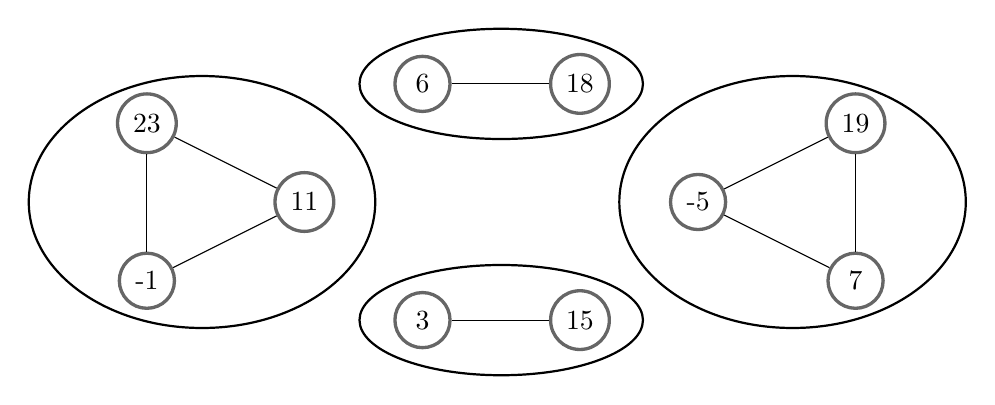
\begin{tikzpicture}[
    node/.style={circle, draw=black!60, very thick, minimum size=7mm},
    ]
    %Nodes
    \node[node] at (-0.5, 0.5) (a) {-1};
    \node[node] at (1.5, 1.5) (b) {11};
    \node[node] at (-0.5, 2.5) (c) {23};
    \node[node] at (6.5, 1.5) (d) {-5};
    \node[node] at (8.5, 0.5) (e) {7};
    \node[node] at (8.5, 2.5) (f) {19};
    \node[node] at (3, 0) (g) {3};
    \node[node] at (5, 0) (h) {15};
    \node[node] at (3, 3) (i) {6};
    \node[node] at (5, 3) (j) {18};
    
    %Lines
    \draw[-] (a) -- (b);
    \draw[-] (a) -- (c);
    \draw[-] (b) -- (c);
    \draw[-] (d) -- (e);
    \draw[-] (d) -- (f);
    \draw[-] (e) -- (f);
    \draw[-] (g) -- (h);
    \draw[-] (i) -- (j);
    
    %elipses
    \draw[thick] (4,0) ellipse (1.8 and 0.7);
    \draw[thick] (4,3) ellipse (1.8 and 0.7);
    \draw[thick] (0.2,1.5) ellipse (2.2 and 1.6);
    \draw[thick] (7.7,1.5) ellipse (2.2 and 1.6);
\end{tikzpicture}
\end{center}
\end{vis}

\subsection{Type-Theoretic view}
This paper focuses on the implementation of quotient types in Coq. Thus, we focus on the Type Theory view of this concept. In Type Theory, quotient types are also induced by some equivalence relation ($\sim$) on underlying type $T$ and denoted $T/\sim$. We denote the equality of elements in the quotient type $T/\sim$ as $a =_\sim b$. Two elements $a$ and $b$ are equal ($a =_\sim b$) if and only if they are in relation ($a \sim b$). Every element of underlying type $T$ is also an element of quotient type $T/\sim$.

Nevertheless, only some functions from underlying type $T$ are well-defined from type $T/\sim$. Function $f : T \rightarrow X$ is well-defined function $f : (T/\sim) \rightarrow X$, if $a \sim b$ implies that $f(a) = f(b)$. Without this restriction, we could differentiate between elements of this same equivalence class by applying an ill-defined function. In other words, applying an ill-defined function breaks the rule that says: $x = y \Rightarrow f(x) = f(y)$.

\section{Quotient types in Coq}
As we mentioned previously, Coq has no built-in method for quotient constructions. Nevertheless, quotients are a helpful concept in formalizing mathematics. Moreover, quotient data types such as sets and multisets are used in many algorithms. Therefore since Coq was introduced, users have been looking for ways to deal with quotients in the Coq language \cite{cicQuotient} \cite{PragmaticQT} \cite{NormalizedTypes}. From those studies, two ways of working with quotient-like types emerged. The first one focuses on replacing the equality relation with an equivalence relation. The second focuses on changing the underlying type so that equivalence implies equality. Both approaches have their downsides and are used interchangeably depending on the situation. In this paper, we focus on the second approach.

\subsection{The setoid approach}
\begin{defi}{Setoid}{def:setoid}
In mathematics, a \emph{setoid} is a set $A$ with an equivalence relation ($\sim$). It is denoted as $(A, \sim)$. In setoids, relation ($\sim$) is meant to be used in place of equality on set A.
\end{defi}
Setoids are concepts known from type theory \cite{SetoidsInTT} \cite{Setoids2}. In Coq, they are often used in the formalization of mathematical concepts. When working with setoids, we need to replace the equality relation in the theorem we are proving with the equivalence relation of the setoid we want to use. It is a minor inconvenience. The bigger one occurs when we want to apply a function on an element of our setoid. In this case, we need to prove that function that is applied is well-defined on setoid (respects equivalence relation). Coq standard library has tools to help users use setoids like rewriting parts of equivalent statements. Unfortunately, it is still far more problematic than using simple equality.

\subsection{The type-based apprach}
Another approach to the lack of quotients in Coq is to define certain types 
where equivalence is the same as equality. This approach usually involves reducing the size of each equivalence class to a single element.

\subsubsection{Subtyping}
This concept will be discussed later in Chapter 2, so the formal definition will be skipped here. Its main idea is to construct a type containing a specific subset of elements. Those elements need to satisfy a particular predicate in case of quotients predicate of being normalized.

\subsubsection{A tailor-made inductive type}
This approach usually gives the best results but only applies to some quotient types. Chapter 4 will show examples of such types based on traces of normalization function. Unfortunately, no general way of getting such type out of the normalization process was not found.

\subsubsection{Additional axioms}
To the Coq system, we can add axioms, and by doing so, we can define quotients similar to other languages like Lean \cite{lean4}. This particular construction will be shown in Chapter 6. Unfortunately, by adding axioms, we lose the computability of our proofs, but usually, we do not need it. However, we must be careful adding axioms since adding contradiction to the Coq system is easy.
\begin{example}{}{ex:ill_defined_mod2}
When dealing with arithmetic modulo 2, we might be tempted to add the following axiom:
\begin{minted}{coq}
Axiom Modulo2 : forall n: nat, n = S (S n).
\end{minted}
It lets us effortlessly rewrite numbers back to their normalized form. Nevertheless, by mistake, we introduced a contradiction. Let us define a function \mintinline{coq}{isZero}, which returns \mintinline{coq}{true} for zero and only zero. Therefore \mintinline{coq}{true = isZero(0) = } \\ \mintinline{coq}{isZero(2) = false}, since \mintinline{coq}{0 = 2}.
\end{example}

\subsubsection{Private inductive types}
Another way of constructing quotients is to use a private inductive type \cite{PrivetInductive}. By using them, we can define the type on which pattern matching outside the module where they are defined is forbidden. If done correctly, it enables us to create constructions like in example \ref{ex:ill_defined_mod2} without introducing contradiction since a user cannot define ill-defined functions.

\section{The equivalence relation induced by a function}
\begin{theo}{The equivalence relation induced by function}{th:equiv_by_fun}
Every function $h: T \rightarrow B$ induces a specific equivalence relation ($\sim_h$) defined below:
$$ \forall x, y \in T, x \sim_h y \iff h(x) = h(y). $$
Moreover, every function $g: B \rightarrow X$ induces a well-defined function $f : T/\sim_h \rightarrow X$ defined as $f = g \circ h$. 
\end{theo}

\begin{proof}{The equivalence relation induced by a function}{proof:equiv_by_fun}
Proof that ($\sim_h$) is an equivalence relation follows directly from the fact that equality on type $B$ is an equivalence relation. \qed \\ 
Given $a, b \in T$ such that $a \sim_h b$. By definition of ($\sim_h$) we know that $h(a) = h(b)$ therefore $f(a) = g(h(a)) = g(h(b)) = f(b)$. So $f$ respects relation $\sim_h$. \qed
\end{proof}
\subsection{Definition of normalization function}
This paper focuses on the particular case of the function $h: T \rightarrow T$, which is idempotent. Such functions we call normalization functions.
\begin{defi}{Normalization function}{def:normalization_function}
\begin{minted}{coq}
Class normalization {A: Type} (f: A -> A) := 
  idempotent : forall x: A, f (f x) = f x.
\end{minted}
\end{defi}
As we know, equivalence relations partition elements into equivalence classes. A normalization function selects a single element from each equivalence class. Elements that have been selected are referred to as normalized or elements in normal form. The idempotence restriction is required to ensure that the normalization function does not change elements already in normal form.

\begin{vis}[B]{Normalization function}{vis:normalization_fuction}
Example of applying normalization function on rational numbers represented as $\mathbb{Z} \times \mathbb{N}$:
\begin{center}
    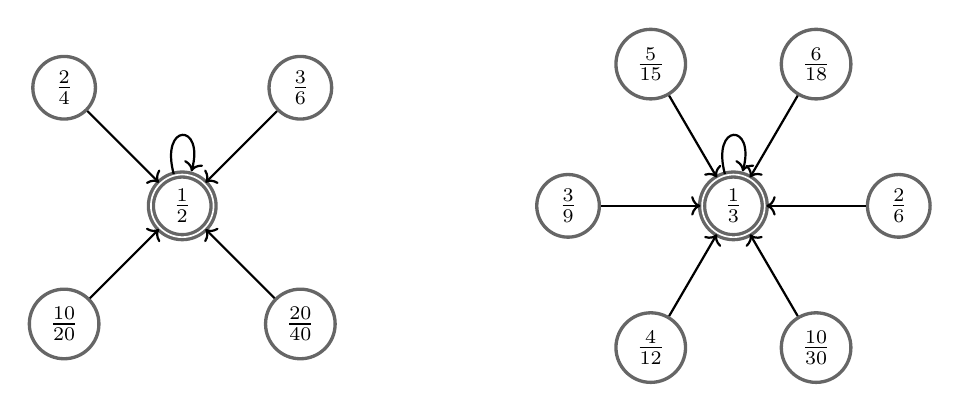
\begin{tikzpicture}[
    node/.style={circle, draw=black!60, very thick, minimum size=0.4}
    ]
    
    %Nodes
    \node[node, double] at (2, 2) (a) {$\frac{1}{2}$};
    \node[node] at (0.5, 3.5) (a0) {$\frac{2}{4}$};
    \node[node] at (3.5, 3.5) (a1) {$\frac{3}{6}$};
    \node[node] at (0.5, 0.5) (a2) {$\frac{10}{20}$};
    \node[node] at (3.5, 0.5) (a3) {$\frac{20}{40}$};

    \node[node, double] at (9, 2) (b) {$\frac{1}{3}$};
    \node[node] at (11.1, 2) (b1) {$\frac{2}{6}$};
    \node[node] at (6.9, 2) (b2) {$\frac{3}{9}$};
    \node[node] at (7.95, 0.2) (b3) {$\frac{4}{12}$};
    \node[node] at (7.95, 3.8) (b4) {$\frac{5}{15}$};
    \node[node] at (10.05, 0.2) (b5) {$\frac{10}{30}$};
    \node[node] at (10.05, 3.8) (b6) {$\frac{6}{18}$};
    
    %Lines
    \path[->, thick] (a) edge [loop above] node {} (a);
    \draw[->, thick] (a0) -- (a);
    \draw[->, thick] (a1) -- (a);
    \draw[->, thick] (a2) -- (a);
    \draw[->, thick] (a3) -- (a);
    
    \path[->, thick] (b) edge [loop above] node {} (b);
    \draw[->, thick] (b1) -- (b);
    \draw[->, thick] (b2) -- (b);
    \draw[->, thick] (b3) -- (b);
    \draw[->, thick] (b4) -- (b);
    \draw[->, thick] (b5) -- (b);
    \draw[->, thick] (b6) -- (b);
    \end{tikzpicture}
\end{center}
\end{vis}

\subsection{Examples of normalization functions}
\begin{example}{Rational numbers}{ex:normalization_fractions}
The standard representation of rational numbers is $\mathbb{Z} \times \mathbb{N}$. For such representation, we can define elements in normal form as irreducible fractions. Therefore normalization function should reduce the fraction by dividing the numerator and the denominator by their greatest common divisor.
\end{example}
\begin{example}{Unordered pair}{ex:normalization_unordered_pirs}
We can define a normalization function for unordered pairs with linear order defined for the underlying type, for example, pairs of natural numbers. Such a function uses the linear order to sort elements of pair. By doing so, the original order of elements in the pair is lost.
\end{example}
\begin{example}{Integers modulo $n$}{ex:normalization_mod}
The normalization function for numbers in arithmetic modulo $n$ is as we expect the operation of calculating modulo.
\end{example}

\section{Quotient types without a normalization function}
Normalization functions are an excellent tool for defining quotient types. By using them, we can select a representative for each equivalence class. Unfortunately, not every quotient type has a computable normalization function. In Set Theory, with the axiom of choice, we can always select a set of representatives of each equivalence relation. Therefore we can always define the normalization function. In Coq, however, we cannot eliminate constructions based on such axiom to define function. 

\subsection{Unordered pairs}
Unordered pair is one of the most basic quotients for which a normalization function does not exist. At least in the most general case, as we learned earlier, if an underlying type has decidable linear order, we can define such a normalization function. Moreover, for some types like, for example, $\mathbb{N} \rightarrow \mathbb{N}$, it is also possible to create such a normalization function based on the computable minimum and maximum, although linear order is not decidable \cite{DefinableQuotients}.

\begin{theo}{}{th:no_normalization_for_unordered_pair}
There is no function $f: (A \times A) \rightarrow A \times A$ for any type A that, for any $\medcircle , \square \in A$ we have $f((\medcircle , \square)) = f((\square, \medcircle))$ and $\medcircle , \square \in f((\medcircle , \square))$ 
\end{theo}

\begin{proof}{}{proof:no_normalization_for_unordered_pair}
Since $f$ is a function for every type $A$, we cannot use values of $\square, \medcircle$ to determine the order of elements. Therefore there are only two functions: $f((\medcircle , \square)) = (\medcircle , \square)$ and $f((\medcircle , \square)) = (\square , \medcircle)$, that satisfy the second property. As can be easily checked, neither satisfies the first property. \qed
\end{proof}

\subsection{Real numbers represented by Cauchy's sequances}
\begin{defi}{Cauchy sequance}{def:cauchy_seq}
Sequence $\{a_n\}_{n\in \mathbb{N}}$ in called \emph{Cauchy sequance} if  elements become arbitrarily close to each other as the sequence progresses \cite{Anal}.
$$
    \textbf{isCauchy}(a) := \forall \epsilon > 0. \exists N \in \mathbb{N}^+. \forall m, n > N. |a_n - a_m| < \epsilon
$$
\end{defi}
Cauchy sequences are often used to construct real numbers out of rational numbers \cite{CauchyReals}. The issue with this construction is that infinitely (even uncountably) many sequences represent a single real number. Using quotients to fix this problem would give us an excellent representation of real numbers for formalizing mathematics. Unfortunately, there is no computable normalization for Cauchy sequences.

\begin{theo}{}{th:no_normalization_for_reals}
There is no computable function $f: (\mathbb{N} \rightarrow \mathbb{Q}) \rightarrow (\mathbb{N} \rightarrow \mathbb{Q})$ that, for any $a, b \in (\mathbb{N} \rightarrow \mathbb{Q})$ we have $\lim_{n \rightarrow \infty}a_n = \lim_{n \rightarrow \infty}b_n \iff f(a) = f(b)$.
\end{theo}

\begin{proof}[G]{}{proof:no_normalization_for_reals}
Let's assume such function $f$ exists.
Let $s_k$ be a sequence consisting of ones to $k$-th place and zeros after. Let $s_\infty$ be a sequence consisting of all ones. \\For all $k$ limit of $s_k$ is zero, and limit of $s_\infty$ is one. Therefore $f(s_k) \not = f(s_\infty)$. If they are different, that means there is a number $t \in \mathbb{N}$ for which $f(s_k)_t \not = f(s_\infty)_t$. So we are able to differentiate between those two in finite time.\\
Let $M$ be an initial state on the Turing machine. Let $c_M(t)$ be zero if the Turing machine finished computations before $t$-th second and one otherwise. This function is computable for every $M$, so we can apply a function $f$ on it and check if the Turing machine with initial state $M$ holts. But the halting problem is undecidable \cite{Undecidable}, so such function $f$ cannot exist. \contradiction
\end{proof}

\subsection{The delay monad}
\begin{defi}{Delay monad}{def:delay_monad}
\begin{minted}{coq}
CoInductive delayed (A : Type) := Delayed {
  state : A + delayed A
}.
\end{minted}
\end{defi}
The delay monad \cite{DelayedMonad} represents computations that may or may not terminate. It is a valuable concept in Coq since it provides an entirely safe way of implementing functions that may not terminate. We want our normalization function to return a value immediately if the computation ever terminates and return infinite delay otherwise. Unfortunately, similar to Cauchy sequences, such normalization function does not exist.
\begin{theo}{}{th:no_normalization_for_delay_monad}
There is no computable function $f: \textrm{delayed} \; A \rightarrow (A + \textrm{unit})$ that, for any terminating computation, returns its final value. Otherwise, it returns an element of unit type.
\end{theo}
\begin{proof}{}{proof:no_normalization_for_delay_monad}
Let's assume that such function $f$ exists. We can model the computation of every partial computable function using a delay monad. Using the normalization function $f$, we can determine if a partial function terminates. But this makes the halting problem decidable, but we know it is undecidable \cite{Undecidable}. Therefore such a normalization function cannot exist. \contradiction
\end{proof}

	
    \chapter{Quotient types and subtypes}
	\section{Czym jest podtypowanie}
Koncept podtypowania jest dosyć intuicyjny. Wyobrazimy sobie na chwilę typy jako zbiory elementów należących do danego typu, wtedy podtyp to będzie podzbiorem naszego pierwotnego typu. Pozwala ono na wyrzucanie z typu wszystkich niepożądanych elementów z naszego typu pierwotnego. Dla przykładu wyobraźmy sobie, że piszemy funkcję wyszukiwania binarnego i jako jej argument chcielibyśmy otrzymać posortowaną listę. W tym celu właśnie możemy użyć podtypowania, wymuszając aby akceptowane były jedynie listy które spełniają predykat posortowania.
\begin{code}
\begin{minted}{coq}
Inductive sig (A : Type) (P : A -> Prop) : Type :=
    exist : forall x:A, P x -> sig P.
    
Record sig' (A : Type) (P : A -> Prop) : Type := exist' {
    proj1' : A;
    proj2' : P proj1';
}
\end{minted}
\caption{Dwie równoważne definicje podtypowania w Coqu.}
\label{sig}
\end{code}
Najbardziej ogólna definicja podtypowania \ref{sig} wymaga wykorzystania typów zależnych, które nie są dostępne w większości języków programowania, stąd też w większości języków programowania na programiście spoczywa obowiązek upewnienie się czy lista jest posortowana, gdyż ekspresywność języka jest zbyt uboga, aby zapisać takie wymagania. Coq w bibliotece standardowej \mintinline{coq}{Coq.Init.Specif} posiada zdefiniowane \mintinline{coq}{sig} wraz z notacją \mintinline{coq}{{a : A | P a}}, która ma przypominać matematyczny zapis $\{x \in A : P(x)\}$. Ta sama biblioteka posiada identyczną konstrukcje, gdzie jednak \mintinline{coq}{(P : A -> Prop)} zostało zamienione na \mintinline{coq}{(P : A -> Type)} jest to uogólniona definicja podtypowania, nazywana sigma typem.
\begin{code}
\begin{minted}{coq}
Inductive sigT (A:Type) (P:A -> Type) : Type :=
    existT : forall x:A, P x -> sigT P Q.
}
\end{minted}
\caption{Definicja definicja sigma typu z biblioteki standardowej Coqa.}
\end{code}
Jest to para zależna w której drugi element pary zależy do pierwszego. Posiada ona również zdefiniowaną notację \mintinline{coq}{{a : A & P}}, nawiązuje ona do tego \mintinline{coq}{a} jest zarówno typu \mintinline{coq}{A} jak i \mintinline{coq}{P}. 
\subsection{Dlaczego w ogóle wspominamy o podtypowaniu?}
Podtypowanie jest to dualna konstrukcja do typów ilorazowych o których mowa w tej pracy. Ten rozdział poświęcamy im z następującego powodu - Coq nie wspiera podtypowania. Nie możemy w żaden inny sposób niż aksjomatem wymusić równości dwóch różnych elementów danego typu. Używanie aksjomatów jest jednak nie praktyczne, gdyż niszczy obliczalność dowodu, a na dodatek bardzo łatwo takimi aksjomatami doprowadzić do sprzeczności w logice Coqa. Dlatego zastąpimy tutaj koncept typów ilorazowych konceptem podtypowania, który będzie wymuszać istnienie jedynie normalnych postaci danej klasy abstrakcji w naszym typie ilorazowym. 
\begin{code}
\begin{minted}{coq}
Record quotient {A: Type} {f: A -> A} (n: normalizing_function f) := {
  val: A;
  proof: val = f val
}.
\end{minted}
\caption{Definicja podtypu kanonicznych postaci względem funkcji normalizującej f.}
\end{code}
Pozwoli nam to na pracę jak na typach ilorazowych korzystając z ograniczonej liczby narzędzi, które dostarcza nam Coq. 
\section{Dualna? Co to oznacza?}
W poprzedniej sekcji wspomnieliśmy, że podtypowanie jest pojęciem dualnym do ilorazów, tu wyjaśnimy co to oznacza. Dualizm jest pojęciem ze świata teorii kategorii, aby zrozumieć tą sekcję wymagana jest bardzo podstawowa wiedza z tego zakresu. Jeśli ktoś jej natomiast nie posiada może spokojnie ją pominąć gdyż stanowi bardziej ciekawostkę niż integralną część tej pracy. Mówiąc formalnie jeśli $\sigma$ jest konstrukcją w teorii kategorii to konstrukcję dualną do niej $\sigma^{\textrm{op}}$ definiujemy poprzez: 
\begin{itemize}
    \item zamianę pojęć elementu początkowego i końcowego nawzajem,
    \item zmianę kolejności składania morfinizmów.
\end{itemize}
Mając to już za sobą możemy powiedzieć prostym językiem, że dualność polega na zmianie kierunku strzałek w naszej konstrukcji. 
\begin{figure}[!htp]
    \centering
    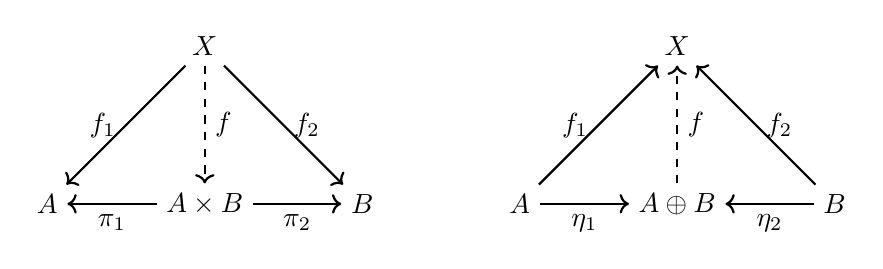
\begin{tikzpicture}[node/.style={circle, draw=black!60, very thick, minimum size=0.4}]
    %Nodes
    \node[] at (0, 0) (pA) {$A$};
    \node[] at (4, 0) (pB) {$B$};
    \node[] at (2, 2) (pX) {$X$};
    \node[] at (2, 0) (pS) {$A \times B$};
    
    \node[] at (6, 0) (cA) {$A$};
    \node[] at (10, 0) (cB) {$B$};
    \node[] at (8, 2) (cX) {$X$};
    \node[] at (8, 0) (cS) {$A \oplus B$};
    
    %Lines
    \draw[->, thick] (pS) -- (pA) node [below, midway] {$\pi_1$};
    \draw[->, thick] (pS) -- (pB) node [below, midway] {$\pi_2$};
    \draw[->, thick] (pX) -- (pA) node [left, midway] {$f_1$};
    \draw[->, thick] (pX) -- (pB) node [right, midway] {$f_2$};
    \draw[->, thick, dashed] (pX) -- (pS) node [right, midway] {$f$};
    
    \draw[->, thick] (cA) -- (cS) node [below, midway] {$\eta_1$};
    \draw[->, thick] (cB) -- (cS) node [below, midway] {$\eta_2$};
    \draw[->, thick] (cA) -- (cX) node [left, midway] {$f_1$};
    \draw[->, thick] (cB) -- (cX) node [right, midway] {$f_2$};
    \draw[->, thick, dashed] (cS) -- (cX) node [right, midway] {$f$};
    
    \end{tikzpicture}
    \caption{Przykład dwóch dualnych konstrukcji. Po lewej stronie widzimy produkt, a po prawej co-produkt. Oba diagramy komutują.}
    \label{fig:fourier_vis}
\end{figure}
Znając to pojęcie możemy zadać sobie pytanie gdzie w ilorazach i podtypowaniu występują jakieś strzałki, których kierunki mielibyśmy zamieniać? Występują mianowicie odpowiednio w pushoutach oraz pullbackach.
\subsection{Czym jest pushout?}
\begin{figure}[!htp]
    \centering
    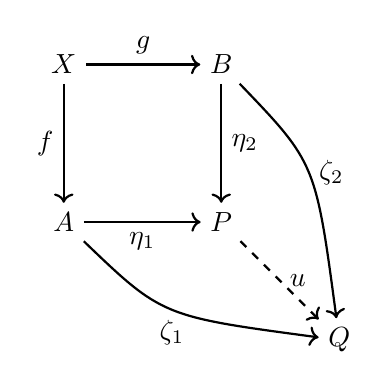
\begin{tikzpicture}[node/.style={circle, draw=black!60, very thick, minimum size=0.4}]
    %Nodes
    \node[] at (0, 0) (a) {$A$};
    \node[] at (2, 0) (p) {$P$};
    \node[] at (0, 2) (x) {$X$};
    \node[] at (2, 2) (b) {$B$};
    
    \node[] at (3.5, -1.5) (q) {$Q$};
    
    %Lines
    \draw[->, thick] (x) -- (a) node [left, midway] {$f$};
    \draw[->, thick] (x) -- (b) node [above, midway] {$g$};
    \draw[->, thick] (a) -- (p) node [below, midway] {$\eta_1$};
    \draw[->, thick] (b) -- (p) node [right, midway] {$\eta_2$};
    \draw[->, thick] (a) .. controls +(1.25, -1.2) .. (q) node [below, midway] {$\zeta_1$};
    \draw[->, thick] (b) .. controls +(1.2, -1.25) .. (q) node [right, midway] {$\zeta_2$};
    \draw[->, thick, dashed] (p) -- (q) node [right, midway] {$u$};
    
    \end{tikzpicture}
    \caption{Diagram definiujący pushout $P$. Diagram komutuje.}
    \label{fig:pushout_def}
\end{figure}
Na rysunku \ref{fig:pushout_def} możemy zobaczyć diagram definiujący pojęcie pushoutu. Widzimy, że powstaje on z pewnych dwóch morfinizmów $f:X \rightarrow A$ oraz $g:X \rightarrow B$. Ponieważ diagram ten komutuje wiemy, że $\eta_1 \circ f = \eta_2 \circ g$. Nasz pushout $P$ jest najlepszym takim obiektem dla którego diagram zachowuje tą własność. Najlepszy definiujemy jako, dla każdego innego obiektu (na diagramie $Q$), dla którego zewnętrzna część ($X, A, B, Q$) diagramu komutuje, istnieje unikatowy (dokładnie jeden) morfizm $u$ z $P$ do $Q$. Warto zaznaczyć, że nie dla każdych dwóch morfinizmów $f:X \rightarrow A$ oraz $g:X \rightarrow B$ istnieje pushout, jeśli jednak istnieje to jest unikatowy z dokładnością do unikatowego izomorfizmu.
\subsection{Przykład pushoutu w kategorii \emph{Set}}
W definicji pushoutu łatwo możemy zobaczyć morfizmy (strzałki), natomiast trudno odnaleźć ilorazy o których jest ta praca. Dużo łatwiej wyrobić swoją intuicję na bardziej przyziemnym przykładzie. Przenieśmy się w tym celu do kategorii \emph{Set}. Oznacza to, że nasze obiekty staną się zbiorami, a morfizmy (strzałki) funkcjami na zbiorach. Na rysunku \ref{fig:pushout_def} możemy zauważyć, że $A$, $B$ oraz $P$ tworzą coś na kształt co-produktu. Zatem warto zacząć definiowanie $P$ właśnie od $A \oplus B$. Wszystko byłoby wszystko dobrze gdyby nie to, że nasz diagram powinien komutować, a więc dla każdego $x \in X$ wiemy, że $\eta_1(f(x)) = \eta_2(g(x))$. Aby to zapewnić musimy utożsamić z sobą $f(x) \sim g(x)$, dla każdego $x \in X$. Dzięki podzieleniu przez tą relację zapewnimy sobie komutowane wewnętrznej części diagramu ($X, A, B, P$). Nie możemy jednak wziąć dowolnej relacji $\sim$ spełniającej ten warunek, gdyż musimy zapewnić istnienie funkcji $u$ do każdego innego zbioru dla którego ten diagram będzie komutował, oznacza to że musi istnieć surjekcja ze zbioru $P$ do $Q$. Z uwagi na komutowanie funkcja $u$ musi spełniać $u \circ \eta_1 = \zeta_1$ oraz $u \circ \eta_2 = \zeta_2$. Nasza relacja równoważności musi zatem być tą najdrobniejszą, aby spełnić ten warunek. Jeśli nasz pushout $P$ jest równy $(A \oplus B) / \sim$ diagram \ref{fig:pushout_def} będzie komutował.  Widzimy zatem, że pushout rzeczywiście ma jakiś związek z typami ilorazowymi, w których to $X$ definiuje które elementy zostaną z sobą utożsamione. 
\subsection{Sklejanie dwóch odcinków w okrąg, czyli pushout}
Rozważyliśmy bardziej przyziemny, lecz dojść abstrakcyjny przykład w kategorii \emph{Set}. Skonstruujmy nieco bardziej wizualny przykład, czyli w naszym przypadku okrąg na rysunku \ref{fig:pushout_circ_def}.
\begin{figure}[!htp]
    \centering
    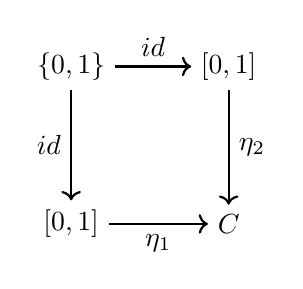
\begin{tikzpicture}[node/.style={circle, draw=black!60, very thick, minimum size=0.4}]
    %Nodes
    \node[] at (0, 0) (a) {$[0, 1]$};
    \node[] at (2, 0) (p) {$C$};
    \node[] at (0, 2) (x) {$\{0, 1\}$};
    \node[] at (2, 2) (b) {$[0, 1]$};
    
    %Lines
    \draw[->, thick] (x) -- (a) node [left, midway] {$id$};
    \draw[->, thick] (x) -- (b) node [above, midway] {$id$};
    \draw[->, thick] (a) -- (p) node [below, midway] {$\eta_1$};
    \draw[->, thick] (b) -- (p) node [right, midway] {$\eta_2$};;
    
    \end{tikzpicture}
    \caption{Diagram definiujący okrąg $C$ używając pushoutu}
    \label{fig:pushout_circ_def}
\end{figure}
Upewnijmy się, iż rzeczywiście $C$ jest topologicznym okręgiem. Wiemy, że aby diagram \ref{fig:pushout_circ_def} komutował $\eta_1(0) = \eta_2(0)$ oraz $\eta_1(1) = \eta_2(1)$. Skleiliśmy zatem z sobą te dwa punkty. Ponieważ $C$ musi być najlepszym obiektem dla którego diagram komutuje, to żadne inne elementy nie mogą być z sobą sklejone, a więc dla każdego $x \in (0, 1)$ wiemy, że $\eta_1(x) \not= \eta_2(x)$. Więc rzeczywiście stworzyliśmy okrąg, z dwóch odcinków oraz dwóch punktów sklejeń. Ta metoda uogólnia się do wyższych wymiarów. Mając dwie $n$-wymiarowe półkule, a następnie sklejając je w wzdłuż kuli ($n-1$)-wymiarowej otrzymamy kulę $n$-wymiarową. 
\subsection{Czym jest pullback?}
Wiedząc jak wygląda pushout oraz wiedząc, że pullback jest pojęciem do niego dualnym każdy powinien być w stanie narysować diagram go definiujący, możemy się mu przyjrzeć na rysunku \ref{fig:pullback_def}.
\begin{figure}[!htp]
    \centering
    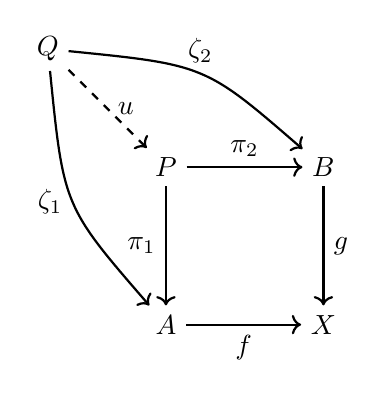
\begin{tikzpicture}[node/.style={circle, draw=black!60, very thick, minimum size=0.4}]
    %Nodes
    \node[] at (0, 0) (a) {$A$};
    \node[] at (0, 2) (p) {$P$};
    \node[] at (2, 0) (x) {$X$};
    \node[] at (2, 2) (b) {$B$};
    
    \node[] at (-1.5, 3.5) (q) {$Q$};
    
    %Lines
    \draw[->, thick] (a) -- (x) node [below, midway] {$f$};
    \draw[->, thick] (b) -- (x) node [right, midway] {$g$};
    \draw[->, thick] (p) -- (a) node [left, midway] {$\pi_1$};
    \draw[->, thick] (p) -- (b) node [above, midway] {$\pi_2$};
    \draw[->, thick] (q) .. controls +(0.2, -2) .. (a) node [left, midway] {$\zeta_1$};
    \draw[->, thick] (q) .. controls +(2, -0.2) .. (b) node [above, midway] {$\zeta_2$};
    \draw[->, thick, dashed] (q) -- (p) node [right, midway] {$u$};
    
    \end{tikzpicture}
    \caption{Diagram definiujący pullback $P$. Diagram komutuje.}
    \label{fig:pullback_def}
\end{figure}
Każdy pullback jest definiowany za pomocą dwóch morfizmów $f: A \rightarrow X$ oraz $g: B \rightarrow X$, które tworzą strukturę przypominającą co-produkt. Z komutacji wiemy, że $f \circ \pi_1 = g \circ \pi_2$. Podobnie jak w przypadku pushoutu, tu również aby $P$ był pullbackiem to musi być najlepszym obiektem, dla którego diagram komutuje. Oznacza to że dla każdego innego (na diagramie $Q$), dla którego zewnętrza część diagramu ($X, A, B, Q$) komutuje to istnieje unikatowy morfizm $u$ z $Q$ do $P$, który oczywiście zachowuje własność komutacji diagramu. Ponownie nie dla każdych dwóch morfizmów $f:A \rightarrow X$ oraz $g:B \rightarrow X$ istnieje pushout, jeśli jednak istnieje to jest unikatowy z dokładnością do unikatowego izomorfizmu.
\subsection{Przykład pullbacku w kategorii \emph{Set}}
Ponownie aby zobaczyć podtypowanie w zdefiniowanym powyżej pullbacku omawiane w tym rozdziale podtypowanie przeniesiemy się do prostszego świata kategorii $Set$, gdzie żyją zbiory oraz funkcje na zbiorach. Jak widzimy na diagramie \ref{fig:pullback_def} struktura $A$, $B$ oraz $P$ przypomina coś na kształt produktu. Zacznijmy więc definiowanie $P$ właśnie od $A \times B$. Wiemy jednak, że aby diagram komutował to dla każdego elementu $p \in P$ musi zachodzić własność $f (\pi_1 (p)) = g (\pi_2(p))$. Ponieważ wstępnie $P = A \times B$ to dla każdej pary $(a, b) \in A \times B$ zachodzi $f(a) = g(b)$. Wystarczy teraz wyrzucić wszystkie elementy nie spełniające tego warunki otrzymując ostatecznie $P = \{(a, b) \in A \times B : f(a) = g(b)\}$. Upewnijmy się jeszcze iż rzeczywiście to jest najlepszy wybór. Weźmy dowolny inny zbiór $Q$ wraz z funkcjami $\zeta_1$ oraz $\zeta_2$ dla którego zewnętrzny diagram \ref{fig:pullback_def} komutuje  i zdefiniujmy morfizm $u$ jako dla każdego $q \in Q$ mamy $u(q) = (\zeta_1(q), \zeta_2(q))$. Ponieważ funkcje $\pi_1$ i $\pi_2$ są zwykłymi projekcjami to własności $\zeta_1 = \pi_1 \circ u$ oraz $\zeta_2 = \pi_2 \circ u$ mamy za darmo, a cała reszta diagramu komutuje z względu na na komutowanie zewnętrznej części diagramu. Możemy na w tym miejscu zauważyć iż rzeczywiście pullback ma związek z podtypowaniem, poprzez wyrzucanie elementów które nie spełniają równości $f(a) = g(b)$.
\subsection{Pary liczb o tej samej parzystości, czyli pullback}
Mamy już za sobą definicję, oraz przykład w kategorii \emph{Set}. Możemy teraz przejść do stworzenia prostego podtypu, w tym przykładzie par liczb całkowitych o tej samej parzystości.  
\begin{figure}[!htp]
    \centering
    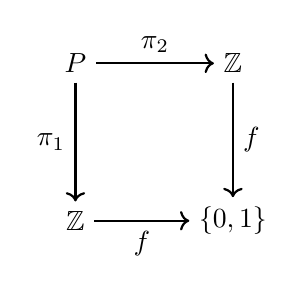
\begin{tikzpicture}[node/.style={circle, draw=black!60, very thick, minimum size=0.4}]
    %Nodes
    \node[] at (0, 0) (a) {$\mathbb{Z}$};
    \node[] at (0, 2) (p) {$P$};
    \node[] at (2, 0) (x) {$\{0, 1\}$};
    \node[] at (2, 2) (b) {$\mathbb{Z}$};
    
    %Lines
    \draw[->, thick] (a) -- (x) node [below, midway] {$f$};
    \draw[->, thick] (b) -- (x) node [right, midway] {$f$};
    \draw[->, thick] (p) -- (a) node [left, midway] {$\pi_1$};
    \draw[->, thick] (p) -- (b) node [above, midway] {$\pi_2$};;
    
    \end{tikzpicture}
    \caption{Diagram definiujący pary liczb całkowitych o tej samej parzystości $P$ używając pullbacku}
    \label{fig:pullback_pair_def}
\end{figure}
Na diagramie \ref{fig:pushout_circ_def} widzimy definicję pullbacku $P$ za pomocą morfizmu $f: \mathbb{Z} \rightarrow \{0, 1\}$, zdefiniowanej jako $f(n) = n \;\textrm{mod}\; 2$. Jak wiemy z poprzedniego przykładu $P = \{(n, m) \in \mathbb{Z} \times \mathbb{Z} : n \;\textrm{mod}\; 2 = m \;\textrm{mod}\; 2 \}$. A więc jest to zbiór to pary dwóch liczb całkowitych, które przystają do siebie molulo 2, czyli mówiąc inaczej mają tą samą parzystość.
\subsection{Konkluzja}
Jak więc zobaczyliśmy na poprzednich przykładach w teorii kategorii pushouty pozwalają nam na wyznaczenie obiektów, które utożsamiają z sobą pewne elementy względem pewnej relacji równoważności, generowanej przez morfizmy. Czyniąc je odpowiednikiem typów ilorazowych. Natomiast pullbacki pozwalają nam stworzyć obiekty z elementami które spełniają pewien zadany przez morfizmy warunek, czyniąc z nich odpowiedniki podtypów. Ponieważ te pojęcia są dualne co możemy zobaczyć na diagramach \ref{fig:pushout_def} oraz \ref{fig:pullback_def}, to możemy mówić o tych pojęciach jako dualnych do siebie nawzajem. 

\section{Unikatowość reprezentacji w podtypowaniu}
Podtypowanie w Coqu nie dostarcza nam jednak niestety tak przyjemnego interfejsu, jak moglibyśmy się spodziewać po matematycznym podejściu do tego konceptu. W teorii zbiorów jesteśmy przyzwyczajeni, że zapisów w stylu $8 \in \{x \in \mathbb{N}: \textrm{even}(x)\} $, w Coq natomiast zapis \mintinline{coq}{8 : {x : nat | even x}} powoduje konflikt typów, gdyż 8 jest typu \mintinline{coq}{nat}, a nie typu \mintinline{coq}{{x : nat | even x}}. Wynika to z  definicji \mintinline{coq}{sig}, gdzie \mintinline{coq}{sig} jest parą zależną w związku z tym, aby skonstruować element tego typu potrzebujemy dwóch składników, wartości oraz dowodu, że ta wartość spełnia spełnia wymagany przez podtypowanie predykat, w tym przypadku \mintinline{coq}{even}.

\begin{code}
\begin{minted}{coq}
Definition even (x: nat) : Prop := exists (t : nat), t + t = x.

Lemma eight_is_even : even 8.
Proof. red. exists 4. cbn. reflexivity. Qed.

Check (exist _ 8 eight_is_even) : {x : nat | even x}.
\end{minted}
\caption{Przykład elementu typu naturalnej liczby parzystej w Coqu}
\end{code}
Takie zdefiniowane podtypowanie rodzi pytanie o unikatowość reprezentacji. Cała koncepcja używania podtypowania do reprezentacji typów ilorazowych opiera się na tym, że będzie istnieć jedynie jeden element w postaci normalnej dla każdej klasy abstrakcji. Istnienie wielu takich elementów różniących się jedynie dowodem uniemożliwiłoby zastosowanie podtypowania do tego celu.
\begin{code}
\begin{minted}{coq}
Theorem uniqnes_of_representation : forall (A : Type) (P : A -> Prop) 
  (x y  : {a : A | P a}), proj1_sig x = proj1_sig y -> x = y.
\end{minted}
\caption{Twierdzenie mówiące o unikalności reprezentacji w podtypowaniu}
\label{uniqnes_of_representation}
\end{code}
Niestety twierdzenia \ref{uniqnes_of_representation} nie można udowodnić w Coq bez dodatkowych aksjomatów, natomiast wersja tego twierdzenia dla \mintinline{coq}{sigT} jest po prostu fałszywa. Pozostaje nam zatem zredukować oczekiwania, lub dodać dodatkowe założenia.
\subsection{Dodatkowe aksjomaty}
Pomimo iż w tej pracy unikamy używania dodatkowych założeń spoza Coq warto rozważyć jakie rezultaty dało by ich zastosowanie. 
\subsubsection{Aksjomat irrelewancji}
Jest to aksjomat mówiący o tym, że nie ma różnicy między dowodami tego samego twierdzenia. 
\begin{code}
\begin{minted}{coq}
Definition Irrelevance := forall (P: Prop) (x y: P), x = y.
\end{minted}
\caption{Definicja irrelewancji w Coqu}
\label{uniqnes_of_representation}
\end{code}
Jak możemy się domyśleć mając tak potężne narzędzie bez trudu możemy udowodnić twierdzenie \ref{uniqnes_of_representation}. 
\begin{code}
\begin{minted}{coq}
Theorem irrelevance_uniqnes : Irrelevance -> forall (A: Type) (P: A -> Prop)
  (x y: {z: A| P z}), proj1_sig x = proj1_sig y -> x = y.
Proof.
  intros Irr A P [x_v x_p] [y_v y_p] H.
  cbn in H; subst.
  apply eq_dep_eq_sig.
  specialize (Irr (P y_v) x_p y_p); subst.
  constructor.
Qed.
\end{minted}
\caption{Dowód unikalności reprezentacji używając irrelewancji w Coq}
\end{code}
Dodatkowo możemy udowodnić, że nasze unikatowość reprezentacji jest tak naprawę równoważna aksjomatowi irrelewacji dowodów.
\begin{code}
\begin{minted}{coq}
Theorem uniqnes_irrelevance : (forall (A: Type) (P: A -> Prop)
  (x y: {z: A| P z}), proj1_sig x = proj1_sig y -> x = y) -> Irrelevance.
Proof.
  intros Uniq P x y.
  specialize (Uniq unit (fun _ => P) (exist _ tt x) (exist _ tt y) eq_refl). 
  refine (eq_dep_eq_dec (A := unit) _ _).
  - intros. left. destruct x0, y0. reflexivity.
  - apply eq_sig_eq_dep. apply Uniq.
Qed.
\end{minted}
\caption{Dowód, że unikalności reprezentacji implikuje irrelewancję w Coq}
\end{code}
\subsubsection{Aksjomat K}
Aksjomat ten został wymyślony przez Habil Streicher w swojej pracy "Investigations Into Intensional Type Theory" \cite{Streicher}. My posłużymy się jego nieco zmodyfikowaną wersją (UIP - uniqueness of identity proofs), która lepiej oddaje konsekwencje jego użycia.
\begin{code}
\begin{minted}{coq}
Definition K := forall (A: Type) (x y: A) (p q: x = y), p = q.
\end{minted}
\caption{Aksjomat K w Coq}
\end{code}
Jest to nieco słabsza wersja aksjomatu irrelewancji, która mówi jedynie o irrelewanjci dowodów równości. Ma on pewną ciekawą konsekwencję, którą została opisana w \cite{Streicher}, a mianowicie pozwala on na zanurzenie równości na parach zależnych w zwykłą równość
\begin{code}
\begin{minted}{coq}
Theorem sig_jnjectivity : K -> forall (A : Type) (P : A -> Prop)
  (a : A) (p q : P a), exist P a p = exist P a q -> p = q.
\end{minted}
\caption{Twierdzenie o zanurzenie równości na parach zależnych w Coq}
\end{code}
Dowód tego twierdzenia pominiemy, lecz można go znaleźć w dodatku Stricher.v. Aksjomat K nie jest równoważny aksjomatowi irrelewacji \cite{gdzieś_dowód_tego} to nie można za jego pomocą udowodnić unikalności reprezentacji w ogólności. W przypadku jednak typów ilorazowych generowanych przez funkcję normalizującą, będziemy potrzebować jedynie predykatów równości.
\begin{code}
\begin{minted}{coq}
Inductive quotient {A: Type} {f: A -> A} (N: normalizing_function f) : Type :=
| existQ : forall x: A, x = f x -> quotient N.

Definition proj1Q {A: Type} {f: A -> A} {N: normalizing_function f} 
(x : quotient N) : A := let (a, _) := x in a.
\end{minted}
\caption{Definicja podtypu postaci kanoniczych generowanych przez funkcję normalizującą f, oraz projekcji dla niego w Coq}
\end{code}
Unikatowość reprezentacji dla tego typu można z łatwością udowodnić wykorzystując aksjomat K.
\begin{code}
\begin{minted}{coq}
Theorem uniqnes_quotient {A: Type} (f: A -> A) (N: normalizing_function f) 
    (q q': quotient N) : K -> (proj1Q q) = (proj1Q q') -> q = q'.
Proof.
  intros K H. 
  destruct q, q'. 
  cbn in *. subst. 
  destruct (K A x0 (f x0) e e0).
  reflexivity.
Qed.
\end{minted}
\caption{Dowód unikalności reprezentacji dla podtypu postaci kanoniczych generowanych przez funkcję normalizującą f w Coq}
\end{code}

Możemy w tym miejscu pójść nawet o krok dalej i zdefiniować, że wszystkie elementy będące w tej samej klasie abstrakcji mają unikalnego reprezentanta, przy założeniu aksjomatu K. Zaczniemy od dowodu że funkcja f rzeczywiście generuje relację równoważności \ref{equivalance_relation} \mintinline{coq}{norm_equiv}.
\begin{code}
\begin{minted}{coq}
Definition norm_equiv {A: Type} (f: A -> A) (N: normalizing_function f)
  (x y: A) : Prop := f x = f y.

Theorem norm_equiv_is_equivalance_relation (A: Type) (f: A -> A)
  (N:normalizing_function f) : equivalance_relation (norm_equiv f N).
Proof.
  unfold norm_equiv. apply equiv_proof.
  - intro x. reflexivity.
  - intros x y H. symmetry. assumption.
  - intros x y z H H0. destruct H, H0. reflexivity.
Qed. 
\end{minted}
\caption{Definicja relacji równoważności generowanej przez funkcję normalizującą w Coq}
\label{norm_equiv}
\end{code}
Mając już definicję jak wygląda ta relacja równoważności możemy przejść do właściwego dowodu.
\begin{code}
\begin{minted}{coq}
Theorem norm_equiv_quotient {A: Type} (f: A -> A) (N: normalizing_function f) 
  (q q': quotient N) : K -> norm_equiv f N (proj1Q q) (proj1Q q') -> q = q'.
Proof.
  intros K H. destruct q, q'.
  cbn in *. unfold norm_equiv in H. 
  assert (x = x0).
  - rewrite e, H, <- e0. reflexivity.
  - subst. destruct (K A x0 (f x0) e e0).
    reflexivity.
Qed.
\end{minted}
\caption{Dowód że wszystkie elementy w tej samej klasie abstrakcji mają wspólnego reprezentanta używając aksjomatu K}
\label{norm_equiv_quotient}
\end{code}
\subsubsection{Związek między tymi aksjomatami}
Jak już wspominaliśmy w ogólności aksjomat K jest szczególnym przypadkiem aksjomatu irrelewancji. Oznacza to że nie są one równoważne, jak ciekawostkę możemy powiedzić, że w świecie z ekstensjonalnością dowodów aksjomat K jest równoważny aksjomatowi irrelewancji.

\begin{code}
\begin{minted}{coq}
Definition Prop_ex : Prop := forall (P Q : Prop), (P <-> Q) -> P = Q.
\end{minted}
\caption{Predykat ekstensjonalności dowodów}
\label{Prop_ex}
\end{code}

\begin{code}
\begin{minted}{coq}
Theorem Irrelevance_K : Irrelevance -> K.
Proof.
  intros Irr A x y. apply Irr.
Qed. 
\end{minted}
\caption{Dowód że irrelewancja implikuje aksjomat K}
\label{Irrelevance_K}
\end{code}

\begin{code}
\begin{minted}{coq}
Theorem K_Irrelevance : Prop_ex -> K -> Irrelevance.
Proof.
  unfold Prop_ex, K, Irrelevance.
  intros Prop_ex K P x y. 
  assert (P = (P = True)).
  - apply Prop_ex. split.
    + intros z. rewrite (Prop_ex P True); trivial. split.
      * trivial.
      * intros _. assumption.
    + intros []. assumption.
  - revert x y. rewrite H. apply K.
Qed. 
\end{minted}
\caption{Dowód, że ekstensjonalność dowodów oraz aksjomat K implikuje irrelewancję}
\label{K_Irrelevance}
\end{code}

\subsection{Wykorzystując \mintinline{coq}{SProp}}
\mintinline{coq}{SProp} jest to uniwersum predykatów z definicyjną irrelewancją. Oznacza to że występuje w nim wbudowany aksjomat irrelewacji i wszystkie dowody tego samego typu można w nim przepisywać, bez dodatkowych założeń. Niestety jest to wciąż eksperymentalna funkcjonalność w Coqu i posiada bardzo ubogą bibliotekę standardową, która nie posiada nawet wbudowanej równości. Posiada natomiast kilka użytecznych konstrukcji:
\begin{description}
    \item[\mintinline{coq}{Box}] - jest to rekord, który pozwala opakować dowolne wyrażenie w \mintinline{coq}{SProp} i przenieść je do świata \mintinline{coq}{Prop},
    \item[\mintinline{coq}{Squash}] - jest to typ induktywny, które jest indeksowany wyrażeniem w \mintinline{coq}{Prop}. Pozwala na przeniesienie dowolnego predykatu do świata \mintinline{coq}{SProp}, co z uwagi na mają ilość konstrukcji w bibliotece standardowej jest bardzo użyteczne,
    \item[\mintinline{coq}{sEmpty}] - jest to odpowiednik \mintinline{coq}{False : Prop}. Posiada on regułę eliminacji z której wynika fałsz,
    \item[\mintinline{coq}{sUnit}] - jest to odpowiednik \mintinline{coq}{True : Prop}. Rrównież pozwala się wydostać z świata \mintinline{coq}{SProp}, za pomocą reguły eliminacji,
    \item[\mintinline{coq}{Ssig}] - jest to odpowiednik \mintinline{coq}{sig}. Ponieważ w tym świecie występuje definicyjna irrelewancja to w bibliotece standardowej wraz z nim otrzymujemy twierdzenie \mintinline{coq}{Spr1_inj}, które mówi o unikalności reprezentacji dla tego typu.
\end{description}
Aby pokazać, że używając podtypowania z \mintinline{coq}{Ssig} również mamy jednego reprezentanta dla klasy abstrakcji musimy zdefiniować najpierw równość oraz nasz typ postaci normalnych.
\begin{code}
\begin{minted}{coq}
Inductive Seq {A: Type} : A -> A -> SProp :=
| srefl : forall x: A, s_eq x x.
\end{minted}
\caption{Typ induktywny równości w \mintinline{coq}{SProp}}
\label{SEq}
\end{code}

\begin{code}
\begin{minted}{coq}
Definition Squotient {A: Type} {f: A->A} (N: normalzation f) : Type :=
  Ssig (fun x : A => Seq x (f x)).
\end{minted}
\caption{Typ postaci normalnych w \mintinline{coq}{SProp}}
\label{SEq}
\end{code}
Mając już podstawowe definicje możemy przejść do właściwego dowodu.

\begin{code}
\begin{minted}{coq}
Theorem only_one_repersentant {A: Type} (f: A -> A) (N: normalzation f) 
  (q q': Squotient N) : norm_equiv f N (Spr1 q) (Spr1 q') -> Seq q q'.
Proof.
  intro H. 
  destruct q, q'. cbn in *. 
  assert (E: Seq Spr1 Spr0).
  - unfold norm_equiv in H. destruct Spr2, Spr3.
    subst. constructor.
  - destruct E. constructor.
Qed.
\end{minted}
\caption{Dowód że wszystkie elementy w tej samej klasie abstrakcji mają wspólnego reprezentanta w \mintinline{coq}{Squotient}}
\label{norm_equiv_quotient}
\end{code}
Korzystanie z \mintinline{coq}{SProp} niesie z sobą jednak poważny problem jakim jest próba przeniesienia predykatu do \mintinline{coq}{Prop}. Gdybyśmy zamienili \mintinline{coq}{Seq} na zwykłą równość (\mintinline{coq}{=}), takim wypadku nie dałoby się udowadniać tego twierdzenia. Dowody w Coqu domyślnie są w uniwersum \mintinline{coq}{Prop} i to w nim chcielibyśmy mieć dowody dla naszych typów ilorazowych. Z uniwersum \mintinline{coq}{SProp} możemy się jedynie wydostać eliminując \mintinline{coq}{sEmpty} lub \mintinline{coq}{sUnit}, co nie gwarantuje możliwości wyprowadzenia analogicznego dowodu w \mintinline{coq}{Prop}.
\subsection{Homotopiczne podejście}
Co jeśli jednak nie chcemy używać dodatkowych aksjomatów i pracować w \mintinline{coq}{Prop}? W takiej sytuacji z ratunkiem przychodzi homotopiczna teoria typów. Jest to relatywnie nowa gałąź matematyki, która zajmuje się dowodami równości w różnych typach\cite{HoTT}. Homotopiczną interpretacją równości jest $\omega$-graf w którym punkty reprezentują elementy typów, a ścieżki dowody równości, ścieżki między ścieżkami dowody równości dowodów równości i tak dalej.
\subsubsection{$N$-typy}
Wprowadza ona różne poziomy uniwersów w których żyją typu w zależności od dowodów równości między nimi. Ich indeksowanie zaczynamy nie intuicyjnie od -2. Opiszmy istotne dla nas nas uniwersa:
\begin{description}
    \item{Contr} - jest to najniższe uniwersum, na poziomie minus dwa. Żyjące w nim typy mają dokładnie jeden element. Przykładem takiego typu jest \mintinline{coq}{unit}.
    \begin{code}
    \begin{minted}{coq}
     Class isContr (A: Type) := ContrBuilder {
       center : A;
       contr  : forall x: A, x = center
     }.
    \end{minted}
    \caption{Klasa typów żyjących w uniwersum Contr.}
    \label{isContr}
    \end{code}
    \item{HProp} - nie mylić z Coqowym \mintinline{coq}{Prop}. Dla typów z tego uniwersum wszystkie elementy są sobie równe. Przykładem mieszkańca tego uniwersum jest \mintinline{coq}{Empty}. Ponieważ nie ma on żadnych elementów, to w trywialny sposób wszystkie jego elementy są równe, ale brak elementów wyklucza bycie w Contr.
    \begin{code}
    \begin{minted}{coq}
     Class isHProp (P : Type) :=
       hProp : forall p q : P, p = q.
    \end{minted}
    \caption{Klasa typów żyjących w uniwersum HProp.}
    \label{isHProp}
    \end{code}
    \item{HSet} - tu również nie ma związku z Coqowym \mintinline{coq}{Set}. Jest to poziom zerowy hierarchii uniwersów. Typy żyjące w tym uniwersum charakteryzują się tym, że jeśli dwa elementy są sobie równe to istnieje tylko jeden dowód tego faktu. Można o tym myśleć jako, że dla tych typów prawdziwy jest aksjomat K. Przykładem takiego typu jest \mintinline{coq}{bool}. Dlaczego jednak ma on unikatowe dowody równości powiemy później. 
    \begin{code}
    \begin{minted}{coq}
     Class isHSet (X : Type) :=
       hSet : forall (x y : X) (p q : x = y), p = q.
    \end{minted}
    \caption{Klasa typów żyjących w uniwersum HSet.}
    \label{isHProp}
    \end{code}
\end{description}
Nie są to jedyne uniwersa. Na kolejnym poziomie żyją typy, dla których dowody równości, między dowodami równości są zawsze tym samym dowodem i tak dalej i tak dalej. Definicję dowolnego uniwersum możemy przyjrzeć się w \ref{IsNType}.
\begin{code}
\begin{minted}{coq}
Inductive universe_level : Type :=
| minus_two  : universe_level
| S_universe : universe_level -> universe_level.

Fixpoint isNType (n : universe_level) (A : Type) : Type :=
match n with
| minus_two => isContr A
| S_universe n' => forall x y: A, isNType n' (x = y)
end.
\end{minted}
\caption{Klasa typów żyjących w $n$-tym uniwersum.}
\label{IsNType}
\end{code}
Jak widzimy typy dowodów równości między elementami typu żyjącego w $(n+1)$-wszym uniwersum żyją na w $n$-tym uniwersum. Aby nabrać nieco więcej intuicji na temat poziomów uniwersów pozwolimy sobie na udowodnienie twierdzenia dotyczącego zawierania się uniwersów. 
\begin{code}
\begin{minted}{coq}
Lemma contr_bottom : forall A : Type, isContr A -> 
  forall x y : A, isContr (x = y).

Theorem NType_inclusion : forall A: Type, forall n : universe_level,
  isNType n A -> isNType (S_universe n) A.
Proof.
  intros A n; revert A.
  induction n; intros A H.
  - cbn in *; intros x y.
    apply contr_bottom; assumption.
  - simpl in *; intros x y.
    apply IHn.
    apply H.
Qed.
\end{minted}
\caption{Dowód, że typu żyjące w $n$-tym uniwersum, żyją też w $(n+1)$-pierwszym uniwersum.}
\label{NType_incusion}
\end{code}
Jak widzimy w twierdzeniu \ref{NType_incusion} każde kolejne uniwersum zwiera w sobie poprzednie. Dowód twierdzenia \mintinline{coq}{contr_bottom} pominiemy tutaj, lecz można się z nim zapoznać w dodatku HoTT.v. Wracając jednak to naszego podtypowania widzimy, że jak długo będziemy się zajmować typami, które żyją w uniwersum HSet, nie będziemy musieli się martwić o dowody równości między elementami tego typu. A więc doskonale nadają się one do bycia pierwotnymi typami dla naszych typów ilorazowych. Pozostaje tylko ustalić które typy należą do tego uniwersum, tu również z pomocą przychodzi homotopiczna teoria typów oraz twierdzenie Hedberg'ga \cite{hedberg_1998}.
\subsubsection{Typy z rozstrzygalną równością}
Na początku warto definiować czym jest rozstrzygalna równość. Dla każdego typu z rozstrzygalną równością istnieje obliczalna (taka która można napisać w Coqu) funkcja która określa czy dwa elementy danego typu są tym samym elementem, czy też nie. 
\begin{code}
\begin{minted}{coq}
Class Decidable (A : Type) :=
  dec : A + (A -> False).

Class DecidableEq (A : Type) :=
  dec_eq : forall x y: A, Decidable (x = y).
\end{minted}
\caption{Definicja rozstrzygalności, oraz rozstrzygalnej równości.}
\label{NType_incusion}
\end{code}
Dobrym przykładem rozstrzygalnego typu jest \mintinline{coq}{bool}. Natomiast rozstrzygalnej równości nie ma na przykład typ funkcji \mintinline{coq}{nat -> nat}. Wspomniane wcześniej twierdzenie Hedberg'ga \cite{hedberg_1998} mówi o tym, że każdy typ z rozstrzygalną równością żyje w uniwersum \emph{HSet}. Dowód zaczniemy od zdefiniowania klasy typów sprowadzalnych.
\begin{code}
\begin{minted}{coq}
Class Collapsible (A : Type) :={ 
  collapse        : A -> A ;
  wconst_collapse : forall x y: A, collapse x = collapse y;
}.
\end{minted}
\caption{Definicja sprowadzalności.}
\label{Collapsible}
\end{code}
Pokażemy, że każdy typ rozstrzygalny jest sprowadzalny \ref{dec_is_collaps}.
\begin{code}
\begin{minted}{coq}
Theorem dec_is_collaps : forall A : Type, Decidable A -> Collapsible A.
Proof.
  intros A eq. destruct eq.
  - exists (fun x => a). intros x y. reflexivity.
  - exists (fun x => x); intros x y.
    exfalso; apply f; assumption.
Qed.
\end{minted}
\caption{Dowód, że każdy typ rozstrzygalny jest sprowadzalny.}
\label{dec_is_collaps}
\end{code}
Szczególnym przypadkiem są więc typy z rozstrzygalną równością, które mają sprowadzalne dowody równości (ścieżki) \ref{PathCollapsible}.
\begin{code}
\begin{minted}{coq}
Class PathCollapsible (A : Type) :=
  path_coll : forall (x y : A), Collapsible (x = y).

Theorem eq_dec_is_path_collaps : forall A : Type, DecidableEq A -> PathCollapsible A.
Proof.
  intros A dec x y. apply dec_is_collaps. apply dec.
Qed.
\end{minted}
\caption{Definicja wraz z dowodem, że każdy typ z rozstrzygalną równością ma sprowadzalne ścieżki.}
\label{PathCollapsible}
\end{code}
Mając już zdefiniowane sprowadzalne ścieżki, potrzebujemy jeszcze szybkiego dowodu, na temat pętli ścieżek \ref{loop_eq}.
\begin{code}
\begin{minted}{coq}
Lemma loop_eq : forall A: Type, forall x y: A, forall p: x = y, 
  eq_refl = eq_trans (eq_sym p) p.
Proof.
  intros A x y []. cbn. reflexivity.
Qed.
\end{minted}
\caption{Dowód, że każda pętla z ścieżek jest \mintinline{coq}{eq_refl}.}
\label{loop_eq}
\end{code}
Mając to już za sobą możemy przejść do właściwego dowodu, że dowolny typ z sprawdzalnymi ścieżkami jest \emph{HSet}'em \ref{path_collaps_is_hset}.
\begin{code}
\begin{minted}{coq}
Theorem path_collaps_is_hset (A : Type) : PathCollapsible A -> isHSet A.
Proof.
  unfold isHSet, PathCollapsible; intros C x y.
  cut (forall e: x=y, e = eq_trans (eq_sym(collapse(eq_refl x))) (collapse e)).
  - intros H p q. 
    rewrite (H q), (H p), (wconst_collapse p q).
    reflexivity.
  - intros []. apply loop_eq.
Qed.
\end{minted}
\caption{Dowód, że każdy typ z sprowadzalnymi ścieżkami jest HSet'em.}
\label{path_collaps_is_hset}
\end{code}
Jak więc widzimy każdy typ z rozstrzygalną równością ma tylko jeden dowód równości między dowolną parą równych sobie elementów. Oznacza to, że bez żadnych dodatkowych aksjomatów możemy udowodnić unikalność reprezentacji dla naszych typów ilorazowych, które mają rozstrzygalny typ pierwotny. Z uwagi na to, iż zdefiniowanie nie trywialnej funkcji normalizującej na typie bez rozstrzygalnej równości jest prawie nie możliwe, typy z rozstrzygalną równością wystarczą nam w tym rozdziale.
\subsubsection{Równość między parami zależnymi}
Podtypowanie w Coqu opiera się na parach zależnych, warto się przyjrzeć w jaki sposób wygląda równość między takimi parami. W przypadku zwykłych par sprawa jest prosta.
\begin{code}
\begin{minted}{coq}
Theorem pair_eq : forall (A B: Type) (a x : A) (b y : B),
  (a, b) = (x, y) -> a = x /\ b = y.
Proof.
  intros. inversion H. split; trivial.
Qed.
\end{minted}
\caption{Charakterystyka równości dla par.}
\label{pair_eq}
\end{code}
Jeśli jednak spróbujemy napisać to samo dla par zależnych otrzymamy błąd wynikający z niezgodności typów dowodów, nawet jeśli pozbędziemy się go ustalając wspólną pierwszą pozycję w parze to nie uda nam się udowodnić iż równość pary implikuje równość drugich elementów tych par, gdyż taka zależność implikowałaby aksjomat K \cite{Streicher}. Aby zrozumieć równość par zależnych musimy najpierw zdefiniować transport.
\begin{code}
\begin{minted}{coq}
Definition transport {A: Type} {x y: A} {P: A -> Type} (path: x = y) 
  (q : P x) : P y :=
match path with
| eq_refl => q
end.
\end{minted}
\caption{Definicja transportu.}
\label{transport}
\end{code}
Transport pozwala na przeniesienie typu \mintinline{coq}{q : P x} wzdłuż ścieżki \mintinline{coq}{path : x = y} do nowego typu \mintinline{coq}{P y}. Pozwala on pozbyć się problemu niezgodności typów w charakterystyce równości na parach zależnych.
\begin{code}
\begin{minted}{coq}
Theorem dep_pair_eq : forall (A: Type) (P: A->Type) (x y: A) (p: P x) (q: P y),
  existT P x p = existT P y q -> exists e: x = y, transport e p = q.
Proof.
  intros A P x y p q H. inversion H.
  exists eq_refl. cbn. trivial.
Qed.
\end{minted}
\caption{Charakterystyka równości dla par zależnych.}
\label{dep_pair_eq}
\end{code}
Jak więc wynika z twierdzenia \ref{dep_pair_eq} równość par zależnych składa się z równości na pierwszych elementów, oraz na równości drugich elementów przetransportowanej wzdłuż pierwszej równości.


    \chapter{Quotient types utilizing subtyping}
	The previous chapter discusses using subtyping to define quotient-like types in Coq. This chapter lists examples of quotients that can be easily defined in this way. It focuses on defining quotients with underlying type living in \mcoq{HSet}. Therefore we are able to use the classical equality definition and work in \mcoq{Prop} sort.
\section{Unordered pairs}
\begin{defi}{Unordered pairs}{def:upair}
In mathematics, an \emph{unordered pair} is a set of the form $\{a, b\}$, where $\{a, b\} = \{b, a\}$ \cite{SetTheorey}. In contrast to the ordered pair where $(a, b) \not= (b, a)$.
\end{defi}
As mentioned in the introduction, there is no normalization function for unordered pairs in the most general case. Therefore we will only discuss the case when the underlying type has full decidable order (definition \ref{def:fullOrd}). Antisymmetry is required to prove the uniqueness of representations, and universality (fullness) is required to define a computable function to construct unordered pair out of two elements.
\begin{defi}{Full decidable order}{def:fullOrd}
\begin{minted}{coq}
Class FullOrd (A : Type) := {
  ord  : A -> A -> bool;
  asym : forall x y : A, ord x y = true -> x = y;
  full : forall x y : A, ord x y = true \/ ord y x = true;
}.
\end{minted}
\end{defi}
\begin{defi}{Unordered pairs in Coq}{def:coqupair}
\emph{Unorder pairs} we can define as a triple of first and second elements and proof that states they are in the correct order.
\begin{minted}{coq}
Record UPair (A : Type) `{FullOrd A} := {
  fst    : A;
  snd    : A;
  sorted : ord fst snd = true;
}.
\end{minted}
\end{defi}
In order to use such defined unordered pairs, we need to define a constructor.
\begin{func}{Constructor of unordered pair}{fun:make_UPair}
\begin{minted}{coq}
Definition make_UPait {A : Type} `{FullOrd A} (x y : A) : UPair A.
Proof.
  destruct (ord x y) eqn:o. 
  - econstructor. apply o.
  - assert (o1: ord y x = true) by
    (destruct (full x y); [rewrite H0 in o; discriminate | auto]).
    econstructor. apply o1.
Qed.
\end{minted}
\end{func}

\subsection{Uniquness of representation}
To talk about the uniqueness of representations, we first need to define the equivalence relation defining this quotient construction. In the case of unordered pairs, if two pairs contain these same elements, they are in quotient defining relation.
\begin{defi}{Equivalence relation for unordered pairs}{def:equiv_upair}
\begin{minted}{coq}
Definition contains {A : Type} `{FullOrd A}  (x y : A)
  (p : UPair A) := (fst p = x /\ snd p = y) \/ 
    (fst p = y /\ snd p = x).

Definition sim {A : Type} `{FullOrd A} (p q : UPair A) :=
  forall x y : A, contains x y p <-> contains x y q. 
\end{minted}
\end{defi}
Having a formal definition of equivalence relation, we can formally verify the claim of unique representation for such defined unordered pairs.
\begin{theo}{Uniquness of representation for unordered pairs}{th:uniq_upair}
\begin{minted}{coq}
Theorem UPair_uniq (A : Type) `{FullOrd A} (p q : UPair A) 
  (x y : A) : contains x y p -> contains x y q -> p = q.
\end{minted}
\end{theo}
\begin{proof}{}{proof:uniq_upair}
\begin{minted}{coq}
intros [(cp1 & cp2) | (cp1 & cp2)] [(cq1 & cq2) | (cq1 & cq2)];
destruct p, q; cbn in *; subst.
2-3: assert (x = y) by (apply asym; assumption); subst.
1-4: f_equal; apply bool_is_hset. Qed.
\end{minted}
As we see, the last part of this proof uses \mcoq{bool_is_hset} theorem. As we know, \mcoq{bool} has decidable equality. According to Hedberg's theorem \ref{th:hedberg}, we know it also has unique identity proofs. Formal proof can be found in \coqsource{Lib/HoTT.v}.
\end{proof}
\section{Finite multisets}
\begin{defi}{Multiset}{def:mset}
In mathematics, a \emph{multiset} (also known as \emph{bag} or \emph{mset}) is a modification of a set concept that allows for multiple instances of elements \cite{SetTheorey}.
\end{defi}
A multiset is another example of a quotient type with applications in everyday programming \cite{MSetApplic}. It is a data structure known from mathematics where the order of elements does not matter. They can be considered as unordered lists. Similar to unordered pairs, there is no normalization function for multisets in the most general case. Therefore we restrict ourselves to underlying types with decidable linear order.
\begin{defi}{Decidable linear order}{def:lo}
\begin{minted}{coq}
Class LinearOrder {A : Type} := {
  ord      : A -> A -> bool;
  anti_sym : forall x y : A, ord x y = true -> ord y x = true ->
               x = y;
  trans    : forall x y z : A, ord x y = true -> 
               ord y z = true -> ord x z = true;
  full     : forall x y : A, ord x y = true \/ ord y x = true;
}.
\end{minted}
\end{defi}
\subsection{The equivalance relation}
Two multisets are in equivalence relation when they contain the same elements in the same quantity. In other words, when they both are permutations of the same list of elements. We propose using an alternative permutation definition. 
\begin{defi}{Permutaion}{def:perm}
\begin{minted}{coq}
Fixpoint count {A : Type} (p : A -> bool) (l : list A) : nat :=
  match l with
  | nil      => O
  | cons h t => if p h then S (count p t) else count p t
  end.

Definition permutation {A : Type} (a b : list A) :=
  forall p : A -> bool, count p a = count p b.
\end{minted}
\end{defi}
This definition works for types with decidable equality, and as we know, decidable linear order implies decidable equality. For such types, the special case of a decidable predicate is the predicate being equal to a specific element. This definition does not require defining all laws of permutations. Therefore, it is easier to use in the context of a sorting function. Proof of the fact that this definition is equivalent to the classic permutation definition for types with decidable equality can be found in \coqsource{Extras/Permutations.v}.
\subsection{The normalization function}
We can use the sorting function as a normalization function for a multiset quotient type. One of the sorting functions with the best asymptotic complexity is merge sort. Moreover, it has a nice functional definition, making it the ideal candidate for a multiset normalization function. We propose a definition using B-trees \cite{Btree}.
\begin{defi}{B-tree}{def:bttree}
\begin{minted}{coq}
Inductive BT (A : Type) : Type :=
| leaf : A -> BT A
| node : BT A -> BT A -> BT A.
\end{minted}
\end{defi}
We also define the insert function that keeps the tree balanced out and the function that converts a list into a balanced-out B-tree.
\begin{func}{Conversion to balanced-out B-tree}{fn:BTins}
\begin{minted}{coq}
Fixpoint BTInsert {A : Type} (x : A) (tree : BT A) :=
  match tree with
  | leaf y => node (leaf x)(leaf y)
  | node l r => node r (BTInsert x l)
  end.

Fixpoint listToBT {A : Type} (x : A) (list : list A) : BT A :=
  match list with
  | nil => leaf x
  | cons y list' => BTInsert x (listToBT y list')
  end.
\end{minted}
\end{func}
As expected, we also need a merging function of two sorted lists.
\begin{func}{Merge}{fn:merge}
\begin{minted}{coq}
Fixpoint merge {A : Type} (ord : A -> A -> bool) (l1 : list A) 
  : (list A) -> list A :=
  match l1 with
  | [] => fun (l2 : list A) => l2
  | h1 :: t1 => fix anc (l2 : list A) : list A :=
    match l2 with
    | [] => l1
    | h2 :: t2 => if ord h1 h2 
                  then h1 :: (merge ord t1) l2
                  else h2 :: anc t2
    end
  end.
\end{minted}
\end{func}
Now we can define the whole merge sort function, using the defined above ancillary functions.
\begin{func}{Merge sort}{fn:mergeSort}
\begin{minted}{coq}
Fixpoint BTSort {A : Type} (ord : A -> A -> bool) 
  (t : BT A) : list A :=
  match t with
  | leaf x => [x]
  | node l r => merge ord (BTSort ord l) (BTSort ord r)
  end. 

Definition mergeSort {A : Type} `{LinearOrder A}
  (l : list A) : list A :=
  match l with
  | [] => []
  | x :: l' => BTSort ord (listToBT x l')
  end.
\end{minted}
\end{func}
\subsection{Uniquness of representation}
\begin{theo}{Uniquness of representation for multisets}{th:uniq_mset}
For every multiset, there is exactly one element in \mcoq{quotient mergeSort} type (defined in \ref{def:subtype_quot}). 
\end{theo}
\begin{proof}{}{proof:uniq_mset}
A sorting function should satisfy two requirements:
\setlist{nolistsep}
\begin{itemize}
    \itemsep 0em 
    \item the output is a sorted list,
    \item the output ts a permutation of input.
\end{itemize}
Proof that the sorting function satisfies then can be found in \coqsource{Lib/MergeSort.v}.\\
Moreover, we can show that for every list of elements, only one permutation of this list is sorted. Proof of this fact is in \coqsource{Lib/Sorted.v}.\\
Combining those facts, we know that sorting is an idempotent function, and there is only one output of this function for each equivalence class. More formal proof can be found in \coqsource{FiniteMultiSet.v}. \qed
\end{proof}
\section{Finite sets}
Sets are a basic construction known from mathematics \cite{SetTheorey}. In a set single element can be present at most one time. Therefore, adding an element to a set that already contains this element does not change the result. Moreover, in sets, the order of elements in sets does not matter. Sets can be considered sorted and deduplicated lists. Like the two previous examples, the most general case sets do not have a normalizing function. Therefore we restrict ourselves to underlying types with decidable linear order (defined in \ref{def:lo}).
\subsection{The equivalance relation}
Two sets are in equivalence relation when they contain the same elements. In other words, for every element in underlying types, if contained in the first one, it has at least one copy in the second. Here we also propose an alternative definition of this relation similar to the previous definition of permutations (defined in \ref{def:perm}).
\begin{defi}{Set equivalance}{def:elem_eq}
\begin{minted}{coq}
Fixpoint any {A : Type} (p : A -> bool) (l : list A) : bool :=
  match l with
  | [] => false
  | (x :: l') => if p x then true else any p l'
  end.

Definition Elem_eq {A : Type} (l l' : list A) : Prop := 
  forall p : A -> bool, any p l = any p l'.
\end{minted}
\end{defi}
For types with decidable equality, it is equivalent to the classical definition using \mcoq{In} predicate. Proof of this fact can be found in \coqsource{Lib/Deduplicated}.
\subsection{The normalization function}
For sets, the normalization function needs to remove duplicates and sort elements. A common approach for such a computer science problem is binary tree \cite{knuth}. This paper also uses it to define a set normalization function.
\begin{defi}{Binary tree}{def:binTree}
\begin{minted}{coq}
Inductive tree (A : Type) : Type :=
| leaf : tree A
| node : A -> tree A -> tree A -> tree A.
\end{minted}
\end{defi}
For purposes of the insert function, we need to use a more convenient interface for comparing elements.
\begin{func}{}{fn:comp}
\begin{minted}{coq}
Definition comp {A : Type} `{LinearOrder A} (x y : A) : comparison 
  := if ord x y then (if ord y x then Eq else Gt) else Lt.
\end{minted}
\end{func}
We can define a function for this data structure that inserts elements into the sorted binary tree if and only if the tree does not already contain it.
\begin{func}[D]{Insertion to binary tree}{fn:binTreeAdd}
\begin{minted}{coq}
Fixpoint insert_tree {A : Type} `{LinearOrder A} (x : A) 
  (t : tree A) : tree A :=
  match t with
  | leaf       => node x leaf leaf
  | node v l r => match comp x v with
                  | Lt => node v (insert_tree x l) r
                  | Eq => node v l r
                  | Gt => node v l (insert_tree x r)
                  end
  end.
\end{minted}
\end{func}
By converting a list into a sorted and deduplicated tree and back to a list, we get a sorted and deduplicated list.
\begin{func}{Deduplicating sort}{fn:DSort}
\begin{minted}{coq}
Fixpoint to_tree {A : Type} `{LinearOrder A} (l : list A) 
  : tree A := 
  match l with
  | []        => leaf
  | (x :: l') => insert_tree x (to_tree l')
  end.

Fixpoint to_list {A : Type} (l : tree A) : list A := 
  match l with
  | leaf       => []
  | node x l r => to_list l ++ [x] ++ to_list r
  end.

Definition DSort {A : Type} `{LinearOrder A} (l : list A) 
  : list A := to_list (to_tree l).
\end{minted}
\end{func}
\subsection{Uniquness of representation}
\begin{theo}{Uniquness of representation for sets}{th:uniq_set}
For every set, there is exactly one element in \mcoq{quotient DSort} type (defined in \ref{def:subtype_quot}). 
\end{theo}
\begin{proof}{}{proof:uniq_set}
A sorting and deduplicating function should satisfy the following requirements:
\setlist{nolistsep}
\begin{itemize}
    \itemsep 0em 
    \item the output is a deduplicated list,
    \item the output is a sorted list,
    \item the output and input contain the same elements.
\end{itemize}
Proof that the function above meets those requirements can be found in \coqsource{Lib/DedupSort.v}.\\
In addition, we know that each set has exactly one sorted and deduplicated list. Proof of this is in  \coqsource{Lib/Deduplicated.v}.\\
From those facts, we conclude that the set normalizing function is idempotent. There is exactly one element in the codomain of this function for each set defining equivalence class. Formal proof can be found in \coqsource{FiniteSet.v}. \qed
\end{proof}

    \chapter{Quotient types as normalization traces}
	This chapter discusses quotient types defined as widely understood traces of normalization functions. The inductive types presented here are inspired by how normalization works for selected quotient types. Some examples reinvented in this chapter are commonly used in Coq, and some are new constructions created for this thesis.
\section{Free monoids}
\begin{defi}{Monoid}{def:monoid}
\emph{Monoid} is an algebraic structure $(\mathbf{A}, \circ)$, where $\mathbf{A}$ is a carrier set and $\circ: \mathbf{A} \rightarrow  \mathbf{A} \rightarrow \mathbf{A}$ is a binary operation and following requirements are fulfilled:
\setlist{nolistsep}
\begin{itemize}
    \itemsep 0em 
    \item there exists a neutral element e $\in \mathbf{A}$, such that $\forall x \in \mathbf{A}. \; e \circ x = x = x \circ e$,
    \item the binary operation $\circ: \mathbf{A} \rightarrow  \mathbf{A} \rightarrow \mathbf{A}$ is associative, that means $\forall x, y, z \in \mathbf{A}. \; x \circ (y \circ z) = (x \circ y) \circ z$.
\end{itemize}
\end{defi}
\begin{example}{Monoid of single argument functions}{ex:funcMonoid}
An algebraic structure of single argument functions ($A \rightarrow A$) with function composition operation is an example of a monoid. Function composition is an associative operation, and identity function is a neutral element of this monoid.
\end{example}
\begin{defi}{Free object}{def:freeObject}
\emph{Free object} $\mathbf{A}$ over algebraic structure is the object where the only equations that hold between elements of the free object are those that follow from the axioms defining this algebraic structure \cite{AbstractAlgebra}.
\end{defi}
\begin{vis}{Equivalent elements of a monoid}{vis:equiv_monoids}
Two equivalent notations of $a \circ b \circ c \circ d$.
\begin{center}
\begin{tikzpicture}[sibling distance=24pt]
    \tikzset{level distance=60pt}
    \Tree [.$\circ$ [.$\circ$ a b ] [.$\circ$ c d ] ]
    \end{tikzpicture}
    \hspace{1cm}
    \begin{tikzpicture}[sibling distance=24pt]
    \Tree [.$\circ$ a [.$\circ$ b [.$\circ$ c [.$\circ$ d e ] ] ] ]
    \end{tikzpicture}
\end{center}
\end{vis}
\begin{example}{Free monoid}{ex:freeMonoid}
Lists of natural numbers are a great example of free monoids. The type of list is often called a type of free monoid. The binary operation in this monoid is the concatenation of lists (\mcoq{++}). Concatenation is associative - the order of concatenation operation does not matter. The empty list is the neutral element in this free monoid.
\begin{minted}{coq}
    [1; 2] ++ [3] = [1] ++ ([2] ++ [3]) = [1] ++ [] ++ [2; 3]
\end{minted}
\end{example}
\subsection{A naive representation}
We are accustomed to list representation of free monoids. Elements of a free monoid we call \emph{strings}. However, not every notation of a string can be expressed as a unique list since, every notation of the same string shares the same list representation. We call the type of every notation of elements of free monoid a naive representation. A first attempt to implement the type of free monoids in Coq for someone unfamiliar with this concept would likely look similar to the definition below. 
\begin{defi}{Naive free monoid representation}{def:naiveMonoid}
\begin{minted}{coq}
Inductive FreeMonoid (A : Type) :=
| leaf : FreeMonoid A
| var  : A -> FreeMonoid A
| op   : FreeMonoid A -> FreeMonoid A -> FreeMonoid A.
\end{minted}
\end{defi}
As we can see in the definition above, we have three constructors: an empty string constructor \mcoq{leaf}, a singleton constructor \mcoq{var}, and a string concatenation constructor \mcoq{op}. 
\subsection{The normalized representation}
As it is easy to notice, naive representation \ref{def:naiveMonoid} is not unique for every string. For example, there are infinitely many representations of the neutral element: \mcoq{leaf}, \mcoq{op leaf leaf} etc. To deal with this problem, we must define a normalized form of strings:
$$
    (a_1 \circ (a_2 \circ (a_3 \circ \dots  \circ (a_n \circ e) \dots ))
$$
As expected, we devised a classic list representation of free monoid. 
\begin{defi}{List as free monoid}{def:list}
\begin{minted}{coq}
Inductive list (A : Type) :=
| nil  : list A
| cons : A -> list A -> list A.
\end{minted}
\end{defi}
The normalization function finds the first element in the naively defined string, puts it as the first constructor, and recursively normalizes the rest of the string. The normalization function returns a natural element if the string is equivalent to a neutral element.
The formal definition of normalization function is not very educative. Therefore, we will skip it. However, we will present a conversion function from a naive representation to a normalized one.
\begin{func}{Conversion from a naive representation to a list}{fn:free_to_list}
\begin{minted}{coq}
Fixpoint free_to_list {A : Type} (m : FreeMonoid A) : list A :=
  match m with
  | leaf   => []
  | var x  => [x]
  | op x y => to_list x ++ to_list y
  end.
\end{minted}
\end{func}
\section{Integers}
Integers are another classic quotient type with many applications in computer science. They result from extending natural numbers to an additive group by adding an opposite element to every natural number. They can be naively represented as a pair of two natural numbers. The first number represents the number of predecessors, and the second represents the number of successors applied to zero.
\subsection{A naive representation}
\begin{defi}{Naive integers representation}{def:naiveInt}
\begin{minted}{coq}
Definition Int : Type := nat * nat.
\end{minted}
\end{defi}
For this representation, we can easily define the addition function by adding the number of predecessors and successors of two numbers.
\begin{func}{Addition of naive integers}{fn:int_add}
\begin{minted}{coq}
Definition int_add (n m : Int) : Int :=
  let (a, b) := n in let (c, d) := m in (a + c, b + d).
\end{minted}
\end{func}
Despite many advantages, this representation is rarely used due to a lack of unique representations. As it is easy to notice, there are infinitely many representations of zero: $1 + (-1)$, $2 + (-2)$, etc. Therefore, we can define a normalization function that will remove redundant pairs of successor and predecessor. After normalization, an integer is made out of either predecessors or successors.
\begin{func}{Normalization of naive integers}{fn:int_norm}
\begin{minted}{coq}
Fixpoint int_norm' (x y : nat) : (nat * nat) :=
  match x, y with
  | S x', S y' => int_norm' x' y'
  | _, _       => (x, y)
  end.

Definition int_norm (p : Int) : Int := 
  let (x, y) := p in int_norm' x y.
\end{minted}
\end{func}
\subsection{The normalized representation}
Having a normalization function for our naive representation, we can, based on this normalization process, define an inductive type of normalized representation. The trace of this normalization process is not very interesting until the last recursion. The length of this process depends entirely on how far from the normalized representation the number is. The last step of the normalization process is in function \ref{fn:int_norm} simplified to \mcoq{_, _}. However, we can expand \mcoq{_, _} to three distinct cases:
\begin{description}
\item[\mcoq{S x', O}] -- for negative \mcoq{S x'},
\item[\mcoq{O, S y'}] -- for positive \mcoq{S y'},
\item[\mcoq{O, O}] -- for zero.
\end{description}
Using this trace, we can define the following inductive type for integers. It is a representation known from Coq's standard library \cite{coqDoc}.
\begin{defi}{Normalized integers representation}{def:Z}
\begin{minted}{coq}
Inductive Z : Type :=
| Pos  : nat -> Z
| Zero : Z
| Neg  : nat -> Z.
\end{minted}
\end{defi}
We can also modify a normalization function \ref{fn:int_norm} to convert naive representations into normalized ones.
\begin{func}{Integers conversion}{fn:int_to_Z}
\begin{minted}{coq}
Fixpoint int_to_Z (x y : nat) : Z :=
  match x, y with
  | S x', S y' => int_to_Z x' y'
  | S x', O    => Neg x'
  | O   , S y' => Pos y'
  | O   , O    => Zero
  end.
\end{minted}
\end{func}
\subsection{Basic operations}
We define some basic operations for the normalized representation of integers \ref{def:Z}. Like natural numbers, starting with successor and predecessor definitions is the best option.
\begin{func}{Successor}{fn:int_succ}
\begin{minted}{coq}
Definition succ (n : Z) : Z :=
  match n with
  | Pos k     => Pos (S k)
  | Zero      => Pos O
  | Neg O     => Zero
  | Neg (S n) => Neg n
  end.
\end{minted}
\end{func}
\begin{func}{Predecessor}{fn:int_pred}
\begin{minted}{coq}
Definition pred (n : Z) : Z :=
  match n with
  | Pos (S n) => Pos n
  | Pos O     => Zero
  | Zero      => Neg O
  | Neg n     => Neg (S n)
  end.
\end{minted}
\end{func}
Both definitions are straightforward but substantially more complicated than the same definitions of operations for naive representations. The fourth case was required to handle the transition to zero in both cases.
\begin{func}{Negation}{fn:int_neg}
\begin{minted}{coq}
Definition neg (n : Z) : Z :=
  match n with
  | Pos k => Neg k
  | Zero  => Zero
  | Neg k => Pos k
  end.
\end{minted}
\end{func}
The definition of negation is simple and does not require a discussion. The next basic operation for integers that we discuss is addition.
\begin{func}{Map $n$ times}{fn:map_n}
\begin{minted}{coq}
Fixpoint map_n {A : Type} (n : nat) (f : A -> A) (x : A) : A :=
  match n with
  | O    => x
  | S n' => f (map_n n' f x)
  end.
\end{minted}
\end{func}
  
\begin{func}{Addition}{fn:Z_add}
\begin{minted}{coq}
Definition add (a b : Z) : Z :=
  match a with 
  | Pos n => map_n (S n) succ b
  | Zero  => b
  | Neg n => map_n (S n) pred b
  end.
\end{minted}
\end{func}
For defining addition, we first need to define an ancillary function that applies some function $n$ times. Using it, we can define addition as applying the successor or predecessor operation several times. Subtraction can be defined as the addition of an opposite number.
\begin{func}{Multiplication}{fn:int_mul}
\begin{minted}{coq}
Definition mul (a b : Z) : Z :=
  match a with 
  | Pos n => map_n (S n) (add b) Zero
  | Zero  => Zero
  | Neg n => neg (map_n (S n) (add b) Zero)
  end.
\end{minted}
\end{func}
The multiplication operation can be defined as adding the same number several times. As we know, the addition and multiplication of integers are commutative and associative. Moreover, multiplication is distributive over addition. Proofs of those facts are too long to be presented in this paper. Though, they are in \coqsource{Integers.v}.
\section{Exotic integers}
Integers representation defined in the previous section is often used in Coq due to its symmetric simple definition and computational properties. For example, the addition has linear complexity to one of the arguments. A small unsatisfactory detail is that we used the inductive type of natural numbers in the definition of integers. The question arises if there is a definition of integers that uses a single inductive type.

\subsection{The alternative normalized representation}
We can define the normalization process in an alternative way. Instead of finishing when we determine if the number is positive or negative, we can continue the process by moving successors from input to output. Of course, this step is de facto an identity function on natural numbers with linear complexity.
\pagebreak
\begin{func}{Alternative normalization}{fn:int_alt_norm}

\begin{minted}{coq}
Fixpoint alt_norm (n m : nat) : nat * nat :=
  match n, m with
  | S n', S m' => alt_norm n' m'
  | O   , S _  => map_n n 
      (fun (i : nat * nat) => let (x, y) := i in (S x, y)) (O, O)
  | O   , _    => map_n m 
      (fun (i : nat * nat) => let (x, y) := i in (x, S y)) (O, O)
  end.
\end{minted}
\end{func}
This unnecessary step changes the trace of the normalization process. Now, after determining the sign of the integer, the length of the trace defines its value. This part of the trace is almost identical for positive and negative numbers. Therefore, they will both use a single constructor \mcoq{Next}. We will use two different nullary constructors for parts of traces where the integer sign is determinated, named \mcoq{Zero} and \mcoq{MinusOne}.
\begin{defi}{Exotic integers representation}{def:Z'}
\begin{minted}{coq}
Inductive Z' : Type :=
| Zero     : Z'
| MinusOne : Z'
| Next     : Z' -> Z'.
\end{minted}
\end{defi}
The \mcoq{Next} constructor is both successor and predecessor depending on the integer to which it is applied. A negative integer is a predecessor; on a zero or positive number, it is a successor. This representation is uncommon. We were not able to find any paper or document in which it was used. This is most likely because the definition from the previous section meets almost all criteria for perfect integer representation.
\begin{func}{Conversion to exotic integrs}{fn:to_Z'}
\begin{minted}{coq}
Fixpoint to_Z' (n m: nat) : Z' :=
  match n, m with
  | S n', S m' => to_Z' n' m'
  | O   , S m' => map_n m' Next MinusOne
  | _   , O    => map_n n Next Zero
  end.
\end{minted}
\end{func}
\subsection{Basic operations}
This definition of integers, however, could be more convenient for defining operations. As we can notice, to determine the sign of a number, we need to check the last constructor. Since our definition uses the same construction for successor and predecessor, even a simple operation of computing the successor of a number has linear complexity.
\begin{func}[D]{Successor}{fn:Z'_succ}
\begin{minted}{coq}
Fixpoint succ (k : Z') : Z' :=
  match k with
  | Zero          => Next Zero
  | MinusOne      => Zero
  | Next Zero     => Next (Next Zero)
  | Next MinusOne => MinusOne
  | Next k'       => Next (succ k')
  end.
\end{minted}
\end{func}
\begin{func}{Predecessor}{fn:Z'_pred}
\begin{minted}{coq}
Fixpoint pred (k : Z') : Z' :=
  match k with
  | Zero          => MinusOne
  | MinusOne      => Next MinusOne
  | Next Zero     => Zero
  | Next MinusOne => Next (Next MinusOne)
  | Next k'       => Next (pred k')
  end.
\end{minted}
\end{func}
Because of those difficulties, we recommend using an intermediate form of naively defined integers \ref{def:naiveInt} or the previous normalized definition of integers representation \ref{def:Z} to carry out computations. The conversion functions can be easily defined. The proof of standard and exotic integers definitions being isomorphic can be found in \coqsource{ExoticInteger.v}.
\section{Positive rational numbers}
In contrast to integers, coming up with a type for rational numbers with unique representation is a challenging task. This section is based on the paper of Yves Bertot \cite{Qplus}, which presents a solution to this problem based on a trace of the Euclidean algorithm.
\subsection{A naive representation}
A naive representation of positive rational numbers is identical to that of integers. It comprises two natural numbers, one for a numerator and one for a denominator. Of course, we cannot divide by zero. Therefore, we can interpret the second number as predecessor of the denominator or accept that some pairs do not represent any number.
\begin{defi}{Naive representation of rational numbers }{def:naiveQ}
\begin{minted}{coq}
Definition Q' : Type := nat * nat.
\end{minted}
\end{defi}
We chose the second option since we want to use an already defined coq operation on natural numbers. As we know from mathematics, there are many notations for the same fraction. $\frac{1}{2}$ or $\frac{2}{4}$ represents the same rational number. Every fraction can be reduced to an irreducible fraction. In order to find this irreducible fraction, we need to divide the numerator and denominator by their greatest common divisor. There are many algorithms to compute this value, but one of the simplest is the Euclidean algorithm.
\begin{func}{Euclidean algorithm}{fn:euclid}
\begin{minted}{coq}
Fixpoint euclid (p q : nat) : nat :=
  match compare p q with
  | Eq => p
  | Gt => euclid (p - q) q
  | Lt => euclid p (q - p)
  end.
\end{minted}
\end{func}
The Euclidean algorithm is based on the law that states $\textrm{gcd}(a, b) = \textrm{gcd}(a - b, b)$ if $a > b$. The observation that will be important for defining a normalized representation is that the trace of this algorithm does not change if both numbers are multiplied by the same positive natural number, as in the example shown below.
\begin{equation}
    \begin{split}
        11k&>5k\\
        (11-5)k=6k&>5k\\
        (6-5)k=k&<4k\\
        k&<3k=(4-1)k\\
        k&<2k=(3-1)k\\
        k&=k=(2-1)k
    \end{split}
\end{equation}
The trace,  defined as inequality signs between values, does not depend on the chosen value $k$. The other observation is that we can compute the input values by knowing the trace of the Euclidean algorithm and the output. Without the output, we can still compute the proportions of input values. Proofs of those statements can be found in \coqsource{Qplus.v}.

\subsection{The normalized representation}
Based on those observations, we define an inductive type for positive rational numbers. It has three constructors: \mcoq{N} when the nominator is greater, \mcoq{D} when the denominator is greater, and \mcoq{One} when both values are the same.
\begin{defi}{Normalized representation}{def:Qplus}
\begin{minted}{coq}
Inductive Qplus : Type :=
| One : Qplus
| N   : Qplus -> Qplus
| D   : Qplus -> Qplus.
\end{minted}
\end{defi}
This construction also provides a nice induction rule for positive rational numbers. The type \mcoq{Qplus} is based on the Euclidean algorithm. Therefore, the conversion function is a slightly modified version of the Euclidean algorithm that returns its trace instead of computing the greatest common divisor. 
\begin{func}{Conversion to Euclidean algorithm trace}{def:qplus_c}
\begin{minted}{coq}
Fixpoint qplus_c' (p q n : nat) : Qplus :=
  match n with
  | O    => One
  | S n' => match compare p q with
            | Eq => One
            | Gt => N (qplus_c' (p - q) q n')
            | Lt => D (qplus_c' p (q - p) n')
            end
  end.

Definition qplus_c (x : Q') : Qplus :=
  let (p, q) := x in qplus_c' p q ((p + q) / gcd p q).
\end{minted}
\end{func}
This function differs from the Euclidean algorithm defined in \ref{fn:euclid} because Coq's termination checker cannot deduce the decreasing argument. Therefore, defining the Euclidean algorithm this way is invalid in Coq (8.14.1). We circumvent this problem by adding an argument (the fuel) that constantly decreases, satisfying the termination condition. In order to not change the algorithm output, we need to set the fuel to be big enough. We know that the Euclidean algorithm needs fewer steps to compute the result than the sum of its inputs. Moreover, as we noticed, multiplying inputs by positive numbers does not change the computations so that we can divide the fuel by the greatest common divisor of inputs.
\begin{func}{Conversion to naive representation}{def:qplus_i}
\begin{minted}{coq}
Fixpoint qplus_i (x : Qplus) : Q' :=
  match x with
  | One  => (1, 1)
  | N x' => let (p, q) := qplus_i x' in (p + q, q)
  | D x' => let (p, q) := qplus_i x' in (p, p + q)
  end.
\end{minted}
\end{func}
The inverse conversion function is an even simpler construction. It is based on $(p - q) + q = p$. Of course, the inverse function does not return the same fraction but the equivalent irreducible fraction. The proof that these functions are inversions up to equivalency can be found in \coqsource{Qplus.v}
\subsection{Extension to the field of rational numbers}
There is a  natural extension to the field of rational numbers. It uses the same construction as the extension of natural numbers to integers (see \ref{def:Z}).
\begin{defi}{Type of normalized rational numbers}{def:FullQ}
\begin{minted}{coq}
Inductive FullQ :=
| QPos  : Qplus -> FullQ
| QZero : FullQ
| QNeg  : Qplus -> FullQ.
\end{minted}
\end{defi}
This type uses defined in this section traces of Euclidean algorithm as the normalized representation of a positive rational number. Therefore, we can extend most of the theorems defined for positive rational numbers to the field extension.
\subsection{Basic operations}
In the field of rational numbers, we can define basic operations. However, the proposed normalized representation is not suited for computations. Therefore, we will perform computations in the homomorphic representation using a pair of two integers. However, only a fraction with a positive denominator represents a valid rational number.
\begin{defi}{Type of naive rational numbers}{def:Q}
\begin{minted}{coq}
Definition Q : Type := Z * Z.
\end{minted}
\end{defi}
In order to use the simpler representation to perform computations, we need to define conversion functions.
\begin{func}{Absolute value}{fn:abs'}
\begin{minted}{coq}
Definition abs' (n : Z) : nat :=
  match n with
  | Pos k => S k
  | Zero  => O
  | Neg k => S k
  end.
\end{minted}
\end{func}
\begin{func}{Embedding natural numbers into integers}{fn:toPos}
\begin{minted}{coq}
Definition toPos (x : nat) : Z :=
  match x with
  | O   => Zero
  | S n => Pos n
  end.
\end{minted}
\end{func}
We first need an absolute value function \ref{fn:abs'} and another function \ref{fn:toPos} that will transform natural number to integer.
\begin{func}{Conversion to the normalized rational number}{fn:fullQ_c}
\begin{minted}{coq}
Definition fullQ_c (q : Q') : FullQ :=
  match q with
  | (Pos n, d) => QPos (qplus_c (S n, abs' d))
  | (Zero , d) => QZero
  | (Neg n, d) => QNeg (qplus_c (S n, abs' d))
  end.
\end{minted}
\end{func}
The conversion function \ref{fn:fullQ_c} works only for fractions with a positive denominator.
\begin{func}{Conversion to the naive rational number}{fn:fullQ_i}
\begin{minted}{coq}
Definition fullQ_i (q : FullQ) : Q :=
  match q with
  | QPos q' => let (n, d) := qplus_i q' in (toPos n, toPos d)
  | QZero   => (Zero, Pos O)
  | QNeg q' => let (n, d) := qplus_i q' in (-toPos n, toPos d)
  end.
\end{minted}
\end{func}
The inverse conversion function \ref{fn:fullQ_i} produces an irreducible fraction with a positive denominator. Having all conversion functions, we can define the addition operation.
\begin{func}{Addition}{fn:Qadd}
\begin{minted}{coq}
Definition Qadd' (x y : Q') : Q' :=
  match x, y with
  | (n, d), (n', d') => (d' * n + d * n', d * d')
  end.

Definition Qadd (x y : FullQ) : FullQ :=
  fullQ_c (Qadd'(fullQ_i x) (fullQ_i y)).
\end{minted}
\end{func}
The additional operation adds numerators of two fractions reduced to a common denominator.
\begin{func}{Negation}{fn:Qneg}
\begin{minted}{coq}
Definition Qneg (q : FullQ) : FullQ :=
  match q with
  | QPos x => QNeg x
  | QZero  => QZero
  | QNeg x => QPos x
  end.
\end{minted}
\end{func}
The negation switches the sign of a rational number. Subtraction can be defined as the addition of a negative number.
\begin{func}{Multiplication}{fn:Qmul}
\begin{minted}{coq}
Definition Qmul' (x y : Q') : Q' :=
  match x, y with
  | (n, d), (n', d') => (n * n', d * d')
  end.

Definition Qmul (x y : FullQ) : FullQ :=
  fullQ_c (Qmul' (fullQ_i x) (fullQ_i y)).
\end{minted}
\end{func}
The multiplication operation multiplies both numerators and denominators.
\begin{func}[D]{Inversion}{fn:Qinv}
\begin{minted}{coq}
Fixpoint Qplus_inv (q : Qplus) : Qplus :=
  match q with
  | N x => D (Qplus_inv x)
  | One => One
  | D x => N (Qplus_inv x)
  end.

Definition Qinv (q : FullQ) : FullQ :=
  match q with
  | QPos x => QPos (Qplus_inv x)
  | QZero  => QZero
  | QNeg x => QNeg (Qplus_inv x)
  end.
\end{minted}
\end{func}
The inversion can be easily computed for the Euclidean algorithm trace by swapping two constructors \mcoq{N} and \mcoq{D}. As we know, the inverse operation switches the numerator and the denominator. By swapping inputs of the Euclidean algorithm, we changed which number was greater at each step. The division can be defined as multiplying the inversion. The proof that rational numbers with those operations are an algebraic field can be found in \coqsource{Extras/FullQ.v}.
\section{Free groups}
In this chapter, we have already learned how to define a free monoid. In this section, we define another free algebraic structure -- free group. Elements of a free group we will call \emph{words}. The construction presented in this subsetion was created for this thesis. The definition of groups and free groups is a common problem in Coq \cite{GroupsCoq} \cite{FreeGroupsCoq}. However, no similar definitions have been found in any paper. 
\begin{defi}{Group}{def:group}
An algebraic structure $(\mathbf{A}, \circ)$, where $\mathbf{A}$ is a carrier set and $\circ: \mathbf{A} \rightarrow  \mathbf{A} \rightarrow \mathbf{A}$ is a binary operation is a \emph{group} \cite{AbstractAlgebra} if:
\setlist{nolistsep}
\begin{itemize}
    \itemsep 0em 
    \item there exists a neutral element e $\in \mathbf{A}$, such that $\forall x \in \mathbf{A}. \; e \circ x = x = x \circ e$.
    \item the binary operation $\circ: \mathbf{A} \rightarrow \mathbf{A} \rightarrow \mathbf{A}$ is associative, that means $\forall x, y, z \in \mathbf{A}. \; x \circ (y \circ z) = (x \circ y) \circ z$.
    \item for every element $x$ there is an inverse element $x^{-1}$, such that $x \circ x^{-1} = x^{-1} \circ x = e$.
\end{itemize}
\end{defi}
\begin{example}{Group of permutations}{ex:permutations}
An interesting example is a group of permutations $S_n$, with permutations composition as a binary operation. The composition of the function (permutation is a function), as we learned in the example of monoid \ref{ex:funcMonoid}, is associative. The constant permutation is the neutral element. We can compute inverse permutation by swapping inputs with outputs for every permutation.
$$
\begin{pmatrix}
    1 & 2 & 3 & 4 & 5 \\
    2 & 3 & 1 & 5 & 4
\end{pmatrix}^{-1}
=
\begin{pmatrix}
    1 & 2 & 3 & 4 & 5 \\
    3 & 1 & 2 & 5 & 4
\end{pmatrix}
$$
\end{example}
\subsection{A naive representation}
We know that the type of free monoids can be represented as the type of lists. The difference between a monoid and a group is that in the group there are inverse elements and in monoid there are not. Therefore, we can naively represent the type of free groups as a type of lists of elements and their signs (information if the element is inverted or not).
\begin{defi}{Naive free group representation}{def:CanonFreeGroup}
\begin{minted}{coq}
Definition NaiveFreeGroup (A : Type) := list (bool * A).
\end{minted}
\end{defi}
As it is easy to notice, this representation is not unique for every element of a free group. Therefore, we need to define a normalization function. In our case, we will remove two elements next to each other with opposite signs.
\begin{defi}{Normalized naive representation}{def:Normalized}
\begin{minted}{coq}
Inductive Normalized {A : Type} : NaiveFreeGroup A -> Prop :=
| NNil   : Normalized []
| NSingl : forall (b : bool) (v : A), Normalized [(b, v)]
| NCons  : forall (b b' : bool) (v w : A) (x : NaiveFreeGroup A), 
            v <> w \/ b = b' -> Normalized ((b', w) :: x) ->
            Normalized ((b, v) :: (b', w) :: x).
\end{minted}
\end{defi}
We need an underlying type with decidable equality to define the normalization function. \pagebreak
\begin{defi}{Decidable equality in Coq}{def:EqDec}
\begin{minted}{coq}
Class EqDec (A : Type) := { 
  eqf         : A -> A -> bool;
  eqf_leibniz : forall x y : A, reflect (x = y) (eqf x y);
}.
\end{minted}
\end{defi}
\begin{coq}{Reflect}{coq:reflect}
Reflect is an inductive type for
relating propositions and booleans \cite{coqDoc}.
\begin{minted}{coq}
Inductive reflect (P : Prop) : bool -> Set :=
| ReflectT : P -> reflect P true
| ReflectF : (P -> False) -> reflect P false.
\end{minted}
\end{coq}
\begin{func}{Normalization function for free group}{fn:normalize}
\begin{minted}{coq}
Fixpoint normalize {A : Type} `{EqDec A} 
  (x : NaiveFreeGroup A) : NaiveFreeGroup A :=
  match x with
  | []           => []
  | (b, v) :: x' => 
      match normalize x' with
      | []              => [(b, v)]
      | (b', v') :: x'' => 
          if andb (eqf v v') (xorb b b')
          then x''
          else (b, v) :: (b', v') :: x''
      end
  end.
\end{minted}
\end{func}
\subsection{The normalized representation}
Based on the normalization process, we will define an inductive type where two of the same elements with opposite signs cannot be next to each other. In order to define this type, we first need to formalize the group in Coq.
\begin{defi}{Type class of groups}{def:coqGroup}
\begin{minted}{coq}
Class Group (A : Type) := GroupDef {
  zero     : A;
  op       : A -> A -> A;
  inv      : A -> A;
  l_op_id  : forall x : A, op zero x = x;
  r_op_id  : forall x : A, op x zero = x;
  l_op_inv : forall x : A, op (inv x) x = zero;
  r_op_inv : forall x : A, op x (inv x) = zero;
  op_assoc : forall x y z : A, op (op x y) z = op x (op y z);
}.

Class EqGroup (A : Type) `{E : EqDec A} `{G : Group A} := {}.

Definition sub {A : Type} `{Group A} (x y : A) := op x (inv y).
\end{minted}
\end{defi}
We can make the following observations if the underlying type is a group. First, we notice that two elements are equal if and only if the difference between them is a neutral element. The second one is that we can define any list as a list of differences between elements. Similar to the normalization process, the list of differences starts with the last element, and then differences from the previous elements are added.
\begin{defi}{Normalized representation of free group}{def:Group}
\begin{minted}{coq}
Inductive NEQuotFreeGroup (A : Type) `{EqGroup A} :=
| Singl  : bool -> A -> NEQuotFreeGroup A
| Switch : forall x : A, Squash (x <> zero) -> 
             NEQuotFreeGroup A -> NEQuotFreeGroup A
| Stay   : A -> NEQuotFreeGroup A -> NEQuotFreeGroup A.

Definition QuotFreeGroup (A: Type) `{EqGroup A} 
  := option (NEQuotFreeGroup A).
\end{minted}
\end{defi}
This inductive type \mcoq{NEQuotFreeGroup}, which contains non-empty normalized words (elements of a free group), is made of three constructors. The first one \mcoq{Singl} is the constructor of a single element word. The second one \mcoq{Switch} is the most interesting because it prevents the existence of two elements next to each other that differ only by a sign. It is used to add an element with the opposite sign. It is made of a difference between the added element and the head of the word and a proof that this difference is not the neutral element. This proof is squashed (see \ref{coq:SProp}), so we do not need to worry about its uniqueness. The third one \mcoq{Stay} is used to add an element with the same sign as the head of the word. It is made of a difference between the added element and the head of the word. This construction cannot be used to define a type of free group with the neutral element since we know that the inverse of neutral elements is a neutral element from the group's laws. Therefore, to define potentially empty words, we need to use a second definition utilizing an option. \mcoq{None} is the empty list constructor.

\begin{example}{Exotic integers}{ex:exotic_group}
    The exotic integer representation (defined in \ref{def:Z'}) is the special case of a free group over the single element type (\mcoq{QuotFreeGroup unit}).
\end{example}

To apply this construction in practice, it is necessary to define conversion functions since the normalized representation is difficult for users to read and write. Therefore, the best approach is to define a word in naive representation and convert it to normalized representation.
\begin{func}{Conversion to normalized representation}{fn:to_quot'}
\begin{minted}{coq}
Fixpoint to_quot' {A : Type} `{EqGroup A} (b : bool) (v: A) 
  (x : NaiveFreeGroup A) : NEQuotFreeGroup A :=
  match x with 
  | []             => Singl b v
  | (b', v') :: x' => 
    if eqb b b' 
    then Stay (sub v v') (to_quot' b' v' x')
    else match eqf_leibniz (sub v v') zero with
         | ReflectF _ p => Switch 
             (sub v v') (squash p) (to_quot' b' v' x')
         | _            => (Singl b v) (* invalid *)
         end
end.
\end{minted}
\end{func}
\begin{func}{Conversion to normalized representation}{fn:to_quot}
\begin{minted}{coq}
Definition to_quot {A : Type} `{EqGroup A} 
  (x : NaiveFreeGroup A) : QuotFreeGroup A :=
match x with
| []           => None
| (b, v) :: x' => Some (to_quot' b v x')
end.
\end{minted}
\end{func}
In the definition of the function \mcoq{to_quot'}, we need to prove that two consecutive elements are distinct when they differ by sign. Fortunately, using \mcoq{reflect} in the decidable equality definition allows us to extract such proof easily. The \mcoq{to_quot} function works correctly only for normalized words, so the result is undefined when mutually inverse elements appear next to each other. In order to create a conversion function for any word, we first need to normalize it, which means composing the conversion function with the normalization function \ref{fn:normalize}.
\begin{func}{Conversion to naive representation}{fn:to_naive'}
\begin{minted}{coq}
Fixpoint to_naive' {A : Type} `{EqGroup A} 
  (x : NEQuotFreeGroup A) : bool * A * list (bool * A) :=
  match x with 
  | Singl b v     => ((b, v), [])
  | Stay v x'     => 
      match to_naive' x' with
      | ((b, v'), y)  => ((b, op v v'), (b, v') :: y)
      end
  | Switch v _ x' => 
      match to_naive' x' with
      | ((b, v'), y)  => ((negb b, op v v'), (b, v') :: y)
      end
  end.
\end{minted}
\end{func}
\begin{func}{Conversion to naive representation}{fn:to_naive}
\begin{minted}{coq}
Definition to_naive {A : Type} `{EqGroup A} 
  (x : QuotFreeGroup A) : NaiveFreeGroup A :=
  match x with
  | None    => []
  | Some x' => let (h, t) := to_naive' x' in h :: t
  end.
\end{minted}
\end{func}
The inverse function \mcoq{to_naive} is simpler. It relies on adding consecutive differences to compute the consecutive values. For the \mcoq{Stay} constructor, the sign of the previous element is copied, while for the \mcoq{Switch} constructor, the opposite sign is used. Since the \mcoq{to_naive'} function deals with non-empty free groups, it returns a non-empty list of elements implemented as a pair consisting of the head and a potentially empty list.


\subsection{Free groups as algebraic groups}
As we know, elements of a free group form a group where the operator is the concatenation of words. The neutral element is the empty word, and the inverse of some word is the same word but reversed and with opposite signs, following the inverse law in groups:
$$
(xy)^{-1} = y^{-1}x^{-1}
$$
We can define the appropriate operations and demonstrate that they satisfy the group laws. These operations can be defined on the normalized representation. However, because the normalized representation is a list of differences, operations such as concatenation or reversing the order are difficult to define and inefficient. Therefore, we will define these operations on the naive representation of free groups, ensuring that the result for normalized arguments is also normalized.
\begin{func}{Insertion}{fn:naive_cons}
\begin{minted}{coq}
Definition naive_cons {A : Type} `{EqGroup A} (b : bool) 
  (v : A) (x : NaiveFreeGroup A) : NaiveFreeGroup A :=
  match x with
  | []            => [(b, v)]
  | (b', v') :: t => if negb (eqf v v') || eqb b b'
                     then (b, v) :: (b', v') :: t
                     else t
  end.
\end{minted}
\end{func}
\begin{func}{Concatenation}{fn:naive_concat}
\begin{minted}{coq}
Fixpoint naive_concat {A : Type} `{EqGroup A} 
  (x y : NaiveFreeGroup A) : NaiveFreeGroup A :=
  match x with
  | []           => y
  | (b, v) :: x' => naive_cons b v (naive_concat x' y)
  end.
\end{minted}
\end{func}
The concatenation of words \mcoq{naive_concat} works similarly to the concatenation of lists, where elements from the first list are transferred to the second. However, in the case of normalized words, adding an element at the beginning of a word can remove its head if it is the same element but with the opposite sign.
\begin{func}{Inversion}{fn:naive_inv}
\begin{minted}{coq}
Fixpoint naive_apinv {A : Type} `{EqGroup A} 
  (x y : NaiveFreeGroup A) : NaiveFreeGroup A :=
  match x with
  | []           => y
  | (b, v) :: x' => naive_apinv x' ((negb b, v) :: y)
  end.

Definition naive_inv {A : Type} `{EqGroup A} 
  (x : NaiveFreeGroup A) : NaiveFreeGroup A := naive_apinv x [].
\end{minted}
\end{func}
Similarly as in case of reversing regular lists, in order to define the inverse function for words (\mcoq{naive_inv}) in linear time, we will use an ancillary function called \mcoq{naive_apinv}. This function transfers elements from one list to another with their signs changed. The result is also normalized since we assume that the input is normalized.
To define these operations for normalized representation, we need to compose functions defined above with conversion functions \ref{fn:to_naive} and \ref{fn:to_quot}. In \coqsource{FreeGroup.v}, we can find proof that the operations defined above satisfy the laws of groups. Moreover, we can also find there proof that there is a single normalized representation for each word.  
\subsection{Free groups as monads}
\begin{defi}{Monad}{def:monad}
\begin{minted}{coq}
Class Monad (M : Type -> Type) := MondadDef {
  pure       : forall {A : Type}, A -> M A;
  bind       : forall {A B : Type}, M A -> (A -> M B) -> M B;
  left_bind  : forall {A B : Type} (f : A -> M B) (x : A), 
                 bind (pure x) f = f x; 
  right_bind : forall {A B : Type} (x : M A), bind x pure = x; 
  comp_bind  : forall {A B C : Type} (f : B -> M C) 
                 (g : A -> M B) (x : M A), bind (bind x g) f = 
                 bind x (fun y => bind (g y) f);
}.
\end{minted}
\end{defi}
Every free group is also a monad and, therefore, a functor. However, for normalized representation, free group is a monad only for types with the group interface \ref{def:coqGroup}. The pure function can be defined as the application of a singleton constructor.
\begin{func}{Pure function}{fn:naive_pure}
\begin{minted}{coq}
Definition naive_pure {A : Type} (x : A) : NaiveFreeGroup A 
  := [(true, x)].
\end{minted}
\end{func}
The bind function for free group is defined as:
$$
    \textrm{bind}_f \; (a_1 \circ a_2^{-1} \circ \dots \circ a_n) = f (a_1) \circ f (a_2) ^{-1} \circ \dots \circ f (a_n)
$$
\pagebreak
\begin{func}{Bind function}{fn:naive_bind}
\begin{minted}{coq}
Fixpoint naive_bind {A B : Type} `{EqGroup A} `{EqGroup B} 
  (x : NaiveFreeGroup A) (f : A -> NaiveFreeGroup B) 
  : NaiveFreeGroup B :=
  match x with
  | []               => []
  | (true , v) :: x' => naive_concat (f v) (naive_bind x' f)
  | (false, v) :: x' => 
      naive_concat (naive_inv (f v)) (naive_bind x' f)
  end.
\end{minted}
\end{func}
The proof that those definitions satisfy monad laws can be found in \coqsource{Extras/FreeGroupMonad.v}.
\section{Finite multisets as lists of differences}
In the previous chapter, we defined a multiset type using subtyping. The question arises if there is a definition of finite multisets that do not require dependant types since this concept is not available in many programming languages. For this purpose, we utilize a list of differences and characterize the underlying types for which it is possible to define such lists. The concept of storing differences and recovering values from them is known in computer science as differential backups \cite{DiffBackups}. However, using it for multiset representation has not been found in any paper read during writing this thesis.
\subsection{An alternative normalization}
We first define a normalization function for multisets of natural numbers to derive a normalized representation.
\begin{func}{Minimal value in the list}{fn:min}
\begin{minted}{coq}
Fixpoint min (h : nat) (l : list nat) : nat :=
  match l with
  | []         => h
  | (h' :: l') => if h' <=? h then min h' l' else min h l'
  end.
\end{minted}
\end{func}
\begin{func}{Subtract constant from every element of the list}{fn:sub_list}
\begin{minted}{coq}
Fixpoint sub_list (s : nat) (l : list nat) : list nat :=
  match l with
  | []        => []
  | (h :: l') => (h - s) :: sub_list s l'
  end.
\end{minted}
\end{func}
\begin{func}{Remove one zero from the list}{fn:rm_one_zero}
\begin{minted}{coq}
Fixpoint rm_one_zero (l : list nat) : list nat :=
  match l with
  | []        => []
  | (h :: l') => if h =? O then l' else h :: rm_one_zero l'
  end.
\end{minted}
\end{func}
\begin{func}[D]{Optimized selection sort}{fn:select_sort}
\begin{minted}{coq}
Fixpoint select_sort' (f : nat) (prev : nat) (l : list nat) 
  : list nat :=
  match f with
  | O    => []
  | S f' =>
    match l with
    | []        => []
    | (h :: l') => 
        let m := min h l' in
        let p := prev + m in
        p :: (select_sort' f' p (rm_one_zero (sub_list m l)))
    end
end.

Definition select_sort (l : list nat) : list nat :=
  select_sort' (length l) O l.
\end{minted}
\end{func}
For normalization, we use a modified selection sort algorithm for natural numbers. The modification optimizes the comparison operations by subtracting the found minimum from each member of the yet-to-be-sorted part of list. Comparing natural numbers in unary representation is linear with respect to the smaller number. As a result, the smaller the numbers on the list, the faster the process of finding the minimum becomes. Since the previously found minimum reduces the values on the sorted list, the list of the consecutive minimums this algorithm finds is a list of consecutive differences of the sorted input list.
\subsection{The normalized representation}
We can generalize this normalization process for all underlying types for which a unique symmetric difference between elements can be computed. For this, an underlying type needs to have a linear order defined. Otherwise, computing a unique minimum would be impossible.
\begin{defi}{Type with computable unique diffrences}{def:Diff}
\begin{minted}{coq}
Class Diff (A : Type) `{E : EqDec A} := {
  D    : Type;
  diff : A -> A -> D;
  add  : A -> D -> A;

  diff_comm    : forall (x y : A), diff x y = diff y x;
  diff_def     : forall (x : A) (d : D), d = diff x (add x d);
  recover      : forall (x y : A), 
    y = add x (diff x y) \/ x = add y (diff x y);
  diff_anti_sym : forall (x : A) (d : D), 
    x = add (add x d) d -> d = diff x x;
  diff_trans   : forall (x y z : A), 
    z = add (add x (diff x y)) (diff y z) -> z = add x (diff x z)
}.
\end{minted}
\end{defi}
In this paper, the definition above has been used. It implies the existence of a linear order without requiring it as a premise. However, it does require a type of symmetric difference -- \mcoq{D}, a function that computes such a difference for two elements -- \mcoq{diff}, and a function that adds the indicated difference to an element -- \mcoq{add}. Additionally, this function should meet five requirements. The first requirement enforces the symmetry of the difference through the commutative law of the difference operation. The second law defines the relationship between the symmetric difference operation and addition. The third one requires that at least one of the elements can be recovered from the symmetric difference. The fourth states that if we add a difference twice and the result does not change, that difference is neutral. The third and fourth laws imply the antisymmetry of the generated order. The fifth one requires our symmetric differences to be transitive, meaning that if we can recover a value by adding two differences with a common end, we can also recover it from the direct difference. We can use this definition to define a linear order: two elements are in a relation if and only if by adding their common difference to the first element we obtain the second element \ref{Diff_is_LO}. The proof of this fact can be found in \coqsource{DifferentialLists.v}.
\begin{defi}{Linear order induced by \mcoq{Diff} type class}{Diff_is_LO}
\begin{minted}{coq}
Global Program Instance Diff_is_LO (A: Type) `{D: Diff A} 
  : LinearOrder A := {
  ord := fun x y => eqf y (add x (diff y x))
}.
\end{minted}
\end{defi}

Having the class of types with computable differences, we can define the type of multisets based on this definition. It is an option on the head of the list and the list of consecutive differences.
\begin{defi}{Normalized representation of multisets}{def:DiffList}
\begin{minted}{coq}
Definition DiffList (A : Type) `{Diff A} :=
  option (A * list D).
\end{minted}
\end{defi}
For this definition, we can define conversion functions.
\begin{func}{Conversion to normalized representation}{fn:to_diff'}
\begin{minted}{coq}
Fixpoint to_diff' {A : Type} `{Diff A} (p : A) (l : list A) 
  : list D :=
  match l with
  | []       => []
  | (h :: t) => diff p h :: to_diff' h t
  end.
\end{minted}
\end{func}
\begin{func}{Conversion to normalized representation}{fn:to_diff}
\begin{minted}{coq}
Definition to_diff {A : Type} `{Diff A} (l : list A) 
  : DiffList A :=
  match l with
  | []       => None
  | (h :: t) => Some (h, to_diff' h t)
  end.
\end{minted}
\end{func}
The function \mcoq{to_diff} computes consecutive differences, assuming that the input is sorted. In order to get a normalized representation for a multiset of any list, we need to compose it with a sort function \ref{fn:mergeSort}.
\begin{func}{Conversion of list of differences to list}{fn:from_diff'}
\begin{minted}{coq}
Fixpoint from_diff' {A : Type} `{Diff A} (x : A) (l : list D) :=
  match l with
  | []      => [x]
  | h :: l' => x :: from_diff' (add x h) l'
  end.
\end{minted}
\end{func}
\begin{func}{Conversion of list of differences to list}{fn:from_diff}
\begin{minted}{coq}
Definition from_diff {A : Type} `{Diff A} (x : DiffList A) 
  : list A :=
  match x with
  | None        => []
  | Some (a, l) => (from_diff' a l)
  end.
\end{minted}
\end{func}
The function \mcoq{from_diff} computes the list of elements by adding all the differences. The proof that for every multiset, exactly one list of differences exists can be found in \coqsource{DifferentialLists.v}.
\subsection{Basic operations}
Having the conversion functions defined, we can use all functions defined for lists as functions for multisets. That means our representation is, for example, a monad (for types that implement \ref{def:Diff}). However, using conversion functions is computationally expensive. Therefore, we define an insertion operation natively on normalized representation.
\begin{func}{Insertion}{fn:add_to_diff'}
\begin{minted}{coq}
Fixpoint add_to_diff' {A : Type} `{Diff A} (x : A) (h : A) 
  (l : list D) : list D :=
  match l with
  | []      => [diff h x]
  | d :: l' => if ord x (add h d)
               then diff h x :: diff x (add h d) :: l'
               else d :: add_to_diff' x (add h d) l'
  end.
\end{minted}
\end{func}
\begin{func}{Insertion}{fn:add_to_diff}
\begin{minted}{coq}
Definition add_to_diff {A : Type} `{Diff A} (x : A) 
  (l : DiffList A) : DiffList A :=
  match l with
  | None        => Some (x, [])
  | Some (h, l) => if ord x h
                   then Some (x, diff x h :: l)
                   else Some (h, add_to_diff' x h l)
  end.
\end{minted}
\end{func}
The function \mcoq{add_to_diff} finds a position where the next value is greater than the adding element. In this position, it computes the difference between the previous value and the adding element and between the adding element and the next value. Next, it replaces the previous difference with two new ones. In function \ref{fn:add_to_diff'}, \mcoq{ord} is the linear order defined by symmetric differences (as defined in \ref{Diff_is_LO}). We can prove that after applying such a function to a list, the new element is present, no element has been removed, and the length of the list has increased by one. The proofs of these facts can also be found in \coqsource{DifferentialLists.v}.


    \chapter{Function types as quotient types}
	In this chapter, we will explore how to define quotient-like types using functions. However, these representations often lead to more problems than solutions. Nonetheless, they are intriguing examples of innovative approaches to quotient types in Coq. These examples are sourced from Coq's set library \cite{coqDoc}. %Better source
\section{Quotient-like functions}
At the beginning of the thesis, we mentioned that it is impossible to define the type of sets and multisets for any arbitrary underlying type. It is true for inductive types, where the order of constructors matters. However, we can utilize the built-in function type. Of course, to reason about the equalities of functions in a sensible manner, we will need to assume the axiom of function extensionality. Introducing this axiom does not introduce any contradictions to the Coq system, so we can safely add it.
\begin{defi}{Function extensionality}{def:FunExt}
\begin{minted}{coq}
Definition FunExt := forall (A B : Type) (f g : A -> B),
    (forall x : A, f x = g x) -> f = g.
\end{minted}
\end{defi}
Without this axiom, two functions are equal if and only if they are intentionally equal, which means they perform computations in the same way. With this axiom, two functions are equal if and only if they give the same results. We can use this property to "forget" the order of elements since the order of computations does not matter as long as it does not change the result.

\section{Sets and multisets}
Knowing this concept, we can define the set as the set characteristic function that decides whether the element is in the set or not.

\begin{defi}{Set as characteristic function}{def:fSet}
\begin{minted}{coq}
Definition set (A : Type) : Type := A -> bool.
\end{minted}
\end{defi}
In contrast to previous definitions of sets, this one lets us define sets with potentially infinitely many elements. We can use this representation to reason about any set with a computable characteristic function. The cost of such a general definition is that some basic functions on set are uncomputable for this representation.
\begin{theo}{Checking emptiness}{th:emptyNotComp}
The function $E : \textrm{set}(X) \rightarrow \{0, 1\}$, which checks whether the set is empty, is uncomputable.
\end{theo}
\begin{proof}{}{proof:emptyNotComp}
Let $E$ be a computable function. For any Turing machine $M$ there exists set $T_M = \{t \in \mathbb{N} : \textrm{after} \; t \; \textrm{steps machine} \; M \; \textrm{is in HALT state}\}$. Every set $T_M$ has a computable characteristic function since checking if the Turing machine halts after a specific number of steps is a computable problem. Checking if $T_M$ is empty is equivalent to checking if the Turning machine ever halts. However, this is an undecidable problem. Therefore, function $E$ is not computable. \phantom{dasd} \contradiction
\end{proof}
Multisets can be defined similarly by replacing codomain type from booleans to natural numbers.
\begin{defi}{Multisets as characteristic function}{def:fMSet}
\begin{minted}{coq}
Definition mset (A : Type) : Type := A -> nat.
\end{minted}
\end{defi}
We can express in this representation only multisets that have finitely many copies of each element of the underlying type. In order to generalize this representation, we need to replace natural numbers with co-natural numbers.
\begin{coq}{Co-natural numbers}{coq:conat}
In Coq, \emph{co-natural numbers} can be defined in the following way:
\begin{minted}{coq}
CoInductive conat : Type := 
| O' : conat
| S' : conat -> conat.
\end{minted}
In contrast to an inductive definition of natural numbers, co-natural numbers are coinductive. That means we define the destructor instead of constructors. Destructor produces from a co-natural number either \mcoq{O'} -- zero or \mcoq{S' n} -- the successor of co-natural number n. Since we use a destructor, we can define a number that is a successor of itself.
\begin{minted}{coq}
CoFixpoint inf : conat := S' inf.
\end{minted}
This number can be called infinity. We can also define any finite number.
\begin{minted}{coq}
Fixpoint toConat (n : nat) : conat :=
  match n with
  | O => O'
  | S n' => S' (toConat n') 
  end.
\end{minted}
\end{coq}
\section{Basic operations}
As we showed in Theorem \ref{th:emptyNotComp}, checking if the set is empty is an undecidable problem. Comparing two sets is an uncomputable operation since we can compare a set to an empty set to check if it is empty. Another missing operation is a mapping operation. We can check emptiness by mapping every element to the element of the unit type if a mapping is computable. Despite those problems, we can still define helpful functions for this set representation. Checking if some element is in a set is trivial since we represent a set as a characteristic function. We can easily define the filtering function.
\begin{func}{Filtering}{fn:set_filter}
\begin{minted}{coq}
Definition set_filter {A : Type} (p : A -> bool) 
  (s : set A) : set A :=
  fun x : A => if p x then s x else false.
\end{minted}
\end{func}
This definition utilizes lazy evaluation. Therefore, potential infinity is not a problem. Similarly, we can define union, intersection, and complement of a set.
\pagebreak
\begin{func}{Union}{fn:set_union}
\begin{minted}{coq}
Definition set_union {A : Type} (s s' : set A) : set A :=
  fun x : A => (s x) || (s' x).
\end{minted}
\end{func}
\begin{func}{Intersection}{fn:set_intersection}
\begin{minted}{coq}
Definition set_intersection {A : Type} (s s' : set A) : set A :=
  fun x : A => (s x) && (s' x).
\end{minted}
\end{func}
\begin{func}{Complement}{fn:set_complement}
\begin{minted}{coq}
Definition set_complement {A : Type} (s : set A) : set A :=
  fun x : A => negb (s x).
\end{minted}
\end{func}
Those operations can also be implemented similarly for multisets using sum and minimum operations. The complement operation is not defined for multisets. The drawback of these lazy computations is that with each subsequent intersection and union, the complexity of the set characteristic function increases. The operation of adding an element to the set can also be defined. However, it requires the underlying type with decidable equality.
\begin{func}{Insertion}{fn:set_add}
\begin{minted}{coq}
Definition set_add {A : Type} `{EqDec A} (a : A) (s : set A)  
  : set A :=
  fun x : A => if eqf x a then true else s x.
\end{minted}
\end{func}
\begin{func}{Conversion to a set}{fn:list_to_set}
\begin{minted}{coq}
Fixpoint list_to_set {A : Type} `{EqDec A} (l : list A) 
  : set A :=
  match l with
  | []        => fun _ => false
  | (h :: l') => set_add h (list_to_set l')
  end.
\end{minted}
\end{func}
Proofs of fundamental properties of those operations can be found in \coqsource{FunctionalQuotient.v}.

    \chapter{Quotient types in selected languages}
	In the previous chapters, we discussed how we can define quotient-like types in Coq. In this chapter, we will examine languages that have built-in support for quotient types. We will learn how they are implemented and whether similar mechanisms can be utilized in Coq.
\section{Lean}
Lean is a proof assistant under development since 2013 \cite{lean4}. It is an open-source tool that verifies program reliability and mathematical theorems, similar to Coq. Due to the similarity of both languages, we will translate Lean's axioms into the Coq language.
\begin{coq}{Differences compared to Coq}{coq:lean}
Unlike Coq, Lean does not require constructivism of theorems \cite{lean4}. It means we are dealing with a system closer to mathematical proofs than programming. Moreover, in Lean, we have definitional irrelevance of propositions. The formal system is based on three axioms:
\begin{itemize}
    \item{Propositional Extensionality}
\begin{minted}{coq}
Axiom prop_ext: forall P Q : Prop, (P <-> Q) <-> (P = Q)
\end{minted}
    \item{Axiom of choice}
\begin{minted}{coq}
Inductive NEmpty (A : Type) : Prop := intro : A -> NEmpty A.
Axiom choice: forall A: Type, NEmpty A -> A.
\end{minted}
    \item{Quotient types}
\begin{minted}{coq}
Axiom Quot : forall {A : Type}, (A -> A -> Prop) -> Type.
\end{minted}
\end{itemize}
One of the main differences between Lean and Coq is the use of classical logic in Lean. Therefore, one might assume that the law of excluded middle should be one of the axioms in this system. However, the three axioms mentioned above are sufficient to derive the law of excluded middle and the extensionality of functions. Extensionality of functions can be derived from quotients, and the law of excluded middle can be derived from the axiom of choice as proposed by Diaconescu \cite{choise}. These proofs can also be found in the Lean standard library under the names \mlean{em} and \mlean{funext}.
\end{coq}
\subsection{Axioms of quotient types}
As we saw in \ref{coq:lean}, quotient types are integral with Lean language. Let us take a closer look at the axioms that define them.
\begin{defi}{Axioms of Lean's quotient types}{def:leanQuot}

The first axiom, named in Lean as \mlean{Quot}, states that quotient type exists for every relation and underlying type.
\begin{minted}{coq}
Axiom Quot : forall {A : Type}, (A -> A -> Prop) -> Type.
\end{minted}
The second axiom, named in Lean as \mlean{Quot.mk}, states that there exists an embedding function that, out of every element of the underlying type, makes an element of quotient type.
\begin{minted}{coq}
Axiom Quot_mk : forall {A : Type} (r : A -> A -> Prop),
  A -> Quot r.
\end{minted}
The third axiom, named in Lean as \mlean{Quot.ind}, provides us with induction law for quotient types. It states that every element of the underlying type is made of an element of the underlying type.
\begin{minted}{coq}
Axiom Quot_ind : 
  forall (A : Type) (r : A -> A -> Prop) (P : Quot r -> Prop),
  (forall a : A, P (Quot_mk r a)) -> forall q: Quot r, P q.
\end{minted}
The fourth axiom, named in Lean as \mlean{Quot.lift}, describes how functions on the underlying type can be applied to the quotient type. It requires that such function respect quotient-defining relation. In Lean, this axiom comes with a rule that application on quotient type works the same way as on the underlying type. In Coq, this rule needs to be added as an additional axiom.
\begin{minted}{coq}
Axiom Quot_lift :
  forall (A : Type) (r : A -> A -> Prop) (B : Type) (f : A -> B),
  (forall a b : A, r a b -> f a = f b) -> Quot r -> B.

Axiom Quot_lift' : forall {A : Type} {r : A -> A -> Prop} 
  {B : Type} (f : A -> B) (P : forall a b: A, r a b -> f a = f b) 
  (x : A), f x = Quot_lift f P (Quot_mk r x).
\end{minted}
The fifth axiom, named in Lean as \mlean{Quot.sound}, states that \mlean{Quot} is indeed a quotient type -- if two elements are in the quotient-defining relation, they share the same element in the quotient type.
\begin{minted}{coq}
Axiom Quot_sound :
  forall (A : Type) (r : A -> A -> Prop) (a b : A),
  r a b -> Quot_mk r a = Quot_mk r b.
\end{minted}
\end{defi}
As we see in the definition \ref{def:leanQuot}, axioms of Lean's quotient types can be expressed in Coq. Therefore, we can use them to add quotient type to the Coq language.
\section{Agda}
Agda is a programming language created to support dependent types \cite{agda}. It originated as an extension of Martin-Löf's type theory \cite{MARTINLOF197573}. Due to these features, Agda can be used as a proof assistant. However, unlike languages such as Coq or Lean, Agda does not have a tactic language, which significantly complicates its use as such. On the other hand, handling dependent types in Agda is at a much higher level than in Coq. Agda can often infer that a particular case is impossible, making the definition of dependent functions much more accessible than in Coq.
\subsection{Higher inductive types}
In standard Agda, there is no built-in mechanism for defining quotient types. Therefore, in this section, we focus on \emph{Cubical} extension that introduces known from homotopic type theory higher inductive types.
\begin{defi}{Higher inductive types}{def:HIT}
\emph{Higher inductive types} (HITs) are a generalization of inductive types that allow constructors to produce not just elements of the defined type but also elements of its iterated identity types \cite{HoTT}.
\end{defi}
\begin{example}{Circle}{ex:circle}
The \emph{circle} is a higher inductive type made out of single element \magda{base} and extra identity proof \magda{loop} \cite{HoTT}. In homotopic interpretation, this is a point with a loop. Therefore, it is called a circle.
\begin{minted}{agda}
data S : Set where
  base : S
  loop : base ≡ base
\end{minted}
\end{example}
\begin{example}{Interval}{ex:interval}
The \emph{interval} is a higher inductive type made out of two elements \magda{left} and \magda{right}, that are connected by single identity proof \magda{segment} \cite{HoTT}.
\begin{minted}{agda}
data interval : Set where
  left    : interval
  right   : interval
  segment : left ≡ right
\end{minted}
\end{example}
\begin{example}{Suspension}{ex:suspension}
The \emph{suspension} is a higher inductive type made out of two elements \magda{north} and \magda{south}, and paths for every element of underlying types \cite{HoTT}.
\begin{minted}{agda}
data susp (A : Set) : Set where
  north : susp A
  south : susp A
  merid : A -> north ≡ south.
\end{minted}
\end{example}
\subsection{Quotient types utilizing HITs}
Higher inductive types solve the fundamental problem of inductive types: the inability to glue equivalent elements. Using inductive types, we can only add new elements via constructors. If two different constructions represent the same value, we need to use some quotient type to glue equivalent elements. Using higher inductive types, we can combine those two steps and add constructors for additional equalities (paths) for the inductive type that is being defined.
\begin{example}{Multiset}{ex:agdaMSet}
\begin{minted}{agda}
data MSet (A : Set) : Set where
  []   : MSet A
  _::_ : A -> MSet A -> MSet A 
  swap : (x y : A) (z : MSet A) -> x :: y :: z ≡ y :: x :: z
\end{minted}
\end{example}
The higher inductive types' downside is that they complicate defining functions since we also need to handle constructors for identity proofs. Otherwise, we could define functions that do not respect identities (paths).
\begin{example}{Union}{ex:agdaMSetUnion}
\begin{minted}{agda}
_ ∪ _ : (xs ys : Bag A) → Bag A
xs ∪ [] = xs
xs ∪ (y :: ys) = y :: (xs ∪ ys)
xs ∪ (swap y y' ys i) = swap y y' (xs ∪ ys) i
\end{minted}
\end{example}
As we see in the example \ref{ex:agdaMSetUnion}, to define a multiset union, we also need to define a case when a multiset is on the path that swaps its heads. For both ends of this path, the result must be the same. Therefore, defining the head function for multisets is impossible.
\begin{coq}{HIT in Coq}{coq:HIT}
In Coq, we can also define higher inductive types. However, they require using private inductive types, proposed by Yves Bertot \cite{PrivetInductive}. Private inductive types let us define the inductive types and hide their definitions. They turn off pattern matching on those inductive types, forcing users to use only exposed functions. Coq's library for homotopy type theory, including higher inductive types \cite{HoTTinCoq}, was created using private inductive types.
\end{coq}

    \chapter{Summary}
	Quotient types hold significant importance in the field of mathematics formalization and theorem proving. Our thesis highlights that the Coq programming language lacks a built-in method to define quotient types. Hence, we must utilize other constructions with some advantageous properties of quotient types. Our thesis mainly focused on quotient-like types, where equality is equivalent to a quotient-defining equivalence relation. We extensively examined different methods of defining such types using normalization functions.

\section{Normalization functions}
The normalization function is a helpful tool for defining quotient-like types. Most quotient types that are frequently used have computable normalization functions that can be utilized for the purpose of defining quotient-like types. However, certain quotient types, such as general unordered pairs or potentially infinite sets, do not have a normalization function. Nevertheless, as demonstrated in the fifth chapter, defining quotient-like types in Coq is possible in such cases, but it usually comes with many disadvantages. For instance, in the case of sets determining whether the set is empty is an undecidable problem. The class of quotient types with computable normalization function is expansive enough to assess various approaches to constructing quotient-like types.
\section{Subtypes}
Subtypes are helpful in the case of defining types with a subset of elements of the underlying type. They are a dual construction to quotient types and they are already available in Coq. They can be easily applied to restrict an underlying type to a subset of normalized elements, assuming we have a normalization function or predicate.

Defining a subtype with only normalized elements is straightforward. However, proving only a single element is in the subtype for every equivalence class is difficult due to the fact that \mcoq{Prop} sort and proof irrelevance axiom are independent. This makes proving the uniqueness of representations in the general case impossible. One possible solution is to add the proof irrelevance axiom to the system. However, there exist other solutions that do not require additional axioms. For instance, we can squash (as in \ref{coq:SProp}) the normalization predicate to ensure that it is inhabited by, at most, a single witness. Nevertheless, this makes proving other subtype properties much more complicated if not impossible. The final solution is to prove that the underlying type of the subtype has unique identity proofs. In such cases, we can define a quotient-like construction and proof that it satisfies the necessary properties for the uniqueness of representations (as in \ref{def:unique_representation}).

Defining quotient-like constructions using subtypes is easy when types have decidable equality and normalization functions. However, defining operations for this construction can be complicated. One solution is to always normalize the result after applying any operation. Another solution is to prove that the result of the operation is normalized if the input is normalized. This approach is recommended if we refrain from using squashed proofs of normalization for subtype definition. It lets us use properties of functions proven on the underlying type without extra effort.
\section{Traces of normalization functions}
In this thesis, a different method for defining quotient-like types is presented. It involves creating tailor-made inductive types using the traces of the normalization process. When constructing these types, it is easy to prove the uniqueness of their representations.

A challenge in this approach is creating a customized inductive type for a quotient type. In chapter four, we give examples of such constructions based on traces of the normalization function. However, generalizing the process of constructing types by examining the normalization function is challenging. Only some steps of the normalization process are relevant for creating a quotient-like type, as most steps depend on which unnormalized form was used.

An example of this problem is the normalization process of integers. The final step alone creates a quotient-like type. The inspiration for this thesis was an inductive type of rational numbers based on traces of the Euclidean algorithm. This approach of using traces of normalization function solved a nontrivial problem. The same can be said for traces of normalization of a free monoid. However, it is uncertain whether there is a connection between the traces of the normalization function and some quotient-like types or whether this was a mere coincidence for those examples.

It is unlikely to find a connection between modified sorting functions and the type of lists of differences. This thesis concludes that there is no general way of deriving a normalized representation based on normalization. However, more research is needed to prove this due to the difficulty of establishing a lack of connection.

One of the challenges with the tailor-made quotient-like types is defining basic operations. Although it was easy to define operations for some types, such as free monoids and integers, it proved difficult for most types. As a result, for defining operations, we had to use a naive representation as an intermediary form. To use operations defined for naive representations, we must demonstrate that they maintain the predicate of normalization.

\section{Related and further works}
This thesis covers numerous concepts related to quotient types in Coq. However, it only includes some constructions. For learning the state-of-the-art practical approach to this problem, we recommend reading \cite{PragmaticQT}. This paper explains how to combine the advantages of setoids and quotient-like types. Another essential paper on this topic is \cite{NormalizedTypes}, which, like this thesis, emphasizes the importance of normalization functions in defining quotient-like types. For those interested in the normalization approach, we also suggest reading \cite{DefinableQuotients}, which discusses the limitations and possibilities of defining quotient types.

The main inspiration for writing this thesis was \cite{Qplus}. This paper describes using traces of the Euclidean algorithm to define the quotient-like type for rational numbers. A similar approach is described in \cite{HereditarilyFS} for Hereditarily Finite Sets. However, we have come to the conclusion that trying to find a universal way of using traces of the normalization function as quotient-like types is a dead end. It is important to note that we can only discover something new by having a small amount of skepticism regarding any information presented to us. Therefore, we encourage readers to verify this conclusion on their own.

We have a couple of recommendations for people interested in quotient types in type theory, regardless of whether they are applicable in Coq or not. Firstly, we suggest reading \cite{DIY_TT}. It is a fantastic introduction to type theory. Moreover, it describes how to define congruence types, a similar concept to quotient types. Next, we recommend reading \cite{Quot_izo}. This paper describes which isomorphisms can and cannot be defined for quotient types. We also suggest reading paper \cite{NuPRL_quot}, which is about quotient types in the NuPRL language. It excellently describes the difference between intentional and extensional approach to quotient types.

\section{Conclusions}
Based on our analysis of various methods for defining quotient-like types in Coq, we have found that their practical usage is limited. Subtypes are more suitable for computational purposes. However, we need to prove the normalization predicate's uniqueness to use them as quotient-like types. Even after that, we need to ensure that the operation preserves the predicate of normalization. This requirement is almost as challenging as proving that the operation respects an equivalence relation. Therefore, sentoids are a better approach in most everyday applications since they can be defined for every equivalence relation without the hardship of defining the normalization function or predicate. However, the downside is that we cannot use equality relations in our prepositions. If we want to use equality relation, a better solution to quotient-ike necessarily types is to incorporate them via axioms, as demonstrated in the sixth chapter, or to use a private inductive type, as in the homotopy type theory (HoTT) library for Coq. Therefore, defining quotient-like types remains an interesting concept, but primarily for academic purposes.

%%%%% BIBLIOGRAFIA
        \bibliographystyle{abbrv}
%	     \bibliographystyle{plabbrv}
	\bibliography{thebibliography}

\end{document}